\documentclass[12pt,a4paper]{article}
\newtheorem{mydef}{Definition}
\newtheorem{theorem}{Theorem}
%packages
\usepackage[dvipsnames]{xcolor}
\usepackage{braket}
\usepackage[utf8]{inputenc}
\usepackage[T1]{fontenc}
\usepackage[english]{babel}
\usepackage{algorithm}
\usepackage{algorithmic}
\usepackage{amsmath}
\usepackage{amsfonts}
\usepackage{amssymb}
\usepackage{graphicx}
\usepackage{hyperref}
\usepackage{tikz}
\usepackage{bbm}
\usepackage{mathtools}
\usetikzlibrary{quantikz}
\usetikzlibrary{arrows.meta}
\usepackage[acronym]{glossaries}
\usepackage[backend=biber,
style=numeric,
citestyle=phys,
]{biblatex} 
\addbibresource{cit.bib}
\usetikzlibrary{positioning,angles,quotes}
\def\layersep{2.5cm}
%glossary 
\makeglossaries
\newacronym{qrl}{QRL}{Quantum Reinforcement Learning}
\newacronym{ai}{AI}{Artificial Intelligence}
\newacronym{drl}{DRL}{Deep Reinforcement Learning}
\newacronym{rl}{RL}{Reinforcement Learning}
\newacronym{qc}{QC}{Quantum Computing}
\newacronym{nn}{NN}{Neural Networks}
\newacronym{mdp}{MDP}{Markov Decision Process}
\newacronym{vqa}{VQA}{Variational Quantum Algorithm}
\newacronym{iid}{i.i.d.}{indipendent identical distributed}
\newacronym{dqn}{DQN}{Deep Q-Network}
\newacronym{sac}{SAC}{Soft-Actor Critic}
\newacronym{a2c}{A2C}{Actor-Critic}
\newacronym{ppo}{PPO}{Proximal Policy Optimization}
\newacronym{qpu}{QPU}{Quantum Processing Unit}
\newacronym{ddpg}{DDPG}{Deep Deterministic Policy Gradient}
%settings
\usepackage[left=3.6cm, bottom=4cm, right=3.6cm, top=4cm]{geometry}
\author{Matteo Conterno}
\title{Prospects of quantum computing approach to reinforcement learning}
%start of document
\begin{document}
	\begin{center}
	\huge
	\textbf{Prospects of quantum computing approach to reinforcement learning}
	
	\vspace{1cm}
	
	\Large
	\textbf{University of Turin and NTTDATA}\\
	\textbf{Matteo Conterno}\\
	\today
	
	\vspace{0.8cm}
	
	\begin{figure}[H]
		\centering
		\includegraphics[width=0.6\linewidth]{img/nttdata}
	\end{figure}
	\begin{figure}[H]
		\centering
		\includegraphics[width=0.6\linewidth]{img/unito}
	\end{figure}
	
	\vspace{0.8cm}
	
	\large
	\textbf{
	\begin{tabular}{rl}
		Relator: & prof.Carlini Alberto\\
		Counter-rapporteur : & prof. Castellani Leonardo
	\end{tabular}
	}
\end{center}

	
	\begin{center}
	\section*{Abstract}
\end{center}
Reinforcement learning is one of three major techniques that allows a model to learn, especially this technique focus on how to create an optimal agent able to reach an objective by interacting with an environment. 
This thesis tries to analyze the possible potentials and advantages that would derive by using quantum circuits with neural networks; 
analyzing and explaining how it is possible to create hybrid algorithms that exploit the advantages of both the classical and quantum algorithm, expanding the applicability not only on simulators, but even on quantum devices such as Rigetti and IonQ's processors through the amazon AWS braket service. 
Lastly it is analyzed how the quantum noise influence an optimal model obtained through a simulator, by testing it on a quantum processor to understand if it is possible to use the hybrid algorithm on the actual devices.
\newline
\begin{center}
	\printglossary
\end{center}

	{
	 	\hypersetup{hidelinks}
		\tableofcontents
	}
    \newpage
	\printglossary[type=\acronymtype]
	\section{Introduction to Deep Reinforcement Learning and Quantum Computing}
%introduction
This section of the thesis is created so that it can give an introduction to the fields of \acrlong{ai}(\acrshort{ai}) specifically to \acrlong{drl}(\acrshort{drl}) and the basis of \acrlong{qc}(\acrshort{qc}) in order to understand afterward the fusion of these two different fields on \acrlong{qrl}(\acrshort{qrl}). If already expert on these subjects fell free to skip at the next section.
%subsection of learnings
\subsection{Approaches of learning}
Currently any kind of \acrshort{ai} requires the following components to learn:
\begin{itemize}
	\item Data
	\item Model
	\item Approach of learning
\end{itemize}
Data is necessary in every \acrshort{ai} model, the amount and quality can heavily influence the ability to correctly and efficiently reach his goal. 
The model is an algorithm that, given some data and a predefined objective, tries to complete his task using some learning approach. In order to check if the model has correctly learned, it will be later tested on unseen data and evaluated to understand if it is able to replicate the performances given a similar dataset.\\
The approach of learning specify how the model can learn to complete his task. At the moment there are three major ways:
\begin{itemize}
	\item \textbf{Supervised learning} : the data is already labeled, this means that we can define when the model is incorrect or correct.
	\item \textbf{Unspervised learning} : the data is not labeled, this means that we can't define easily when the model is correct or incorrect and the model must uncover some pattern.
	\item \textbf{Reinforcement learning} : an agent interact with the environment in order to become the most optimal agent to complete the task.
\end{itemize}
This thesis will focalize mainly on the reinforcement learning approach and especially on the \acrfull{drl} which uses \acrfull{nn} to define the most optimal agent.
In this thesis the focus is on what kind of advantage can be obtained by using a quantum algorithm such as \acrfull{vqa}, this technique can be even used in other context and applications. Futhermore it has been demostrated that \acrshort{vqa} and \acrshort{nn} share some similarities and properties. The main drawback is the fact that when a \acrshort{vqa} is trained on a classical device, there is a major overhead of time due to simulation of the quantum circuit implemented and the number of qubits is limited.
%sub section of reinforcement learning
\subsection{Reinforcement Learning}
As said earlier a reinforcement learning approach consist of creating the most optimal agent able to complete a predefined task by interacting with the environment and taking some action. Questions arises about: how can be defined if an action is good or bad? How to model a dynamic environment? The answer is given by using a statistical model called \acrfull{mdp} .
\subsubsection{Markov Decision Process}
In order to model a dynamic environment where an action can influence the sistem it is necessary to use the \acrfull{mdp} which is an extension of Markov chains; these are a stochastic model that is able to describe a sequence of possible events that satisfy the Markov propriety, that is each event depends only on the previous event.\\
It is necessary to note that an \acrshort{mdp} is based on Markov Chains that not only model the states, but even the time and this can be defined as continuous or discretized.
\acrshort{mdp} is an extension of Markov Chains because the agent can influence the state of environment and outcome, so a framework is necessary to define even his decisions and their consequences. An \acrshort{mdp} is defined as a 4-tuple containing the following elements:
\begin{itemize}
	\item $S$ : set of states
	\item $A$ : set of actions
	\item $P_a (s, s') = Pr(s_{t+1} = s' \vert s_{t} = s)$ : is the transition probability of going from state $s$ to $s'$ by taking an action $a$
	\item $R_{a}(s,s')$ is the immediate reward obtained by transitioning from state $s$ to $s'$ by action $a$
\end{itemize}
The difference with a Markov chains is the presence of $P_a (s, s')$ and $R_{a}(s,s')$ which are necessary for the decision process, to see an example graph of and MDP see Figure \ref{fig:mdpgraph}.
\begin{figure}[!ht]
	\centering
	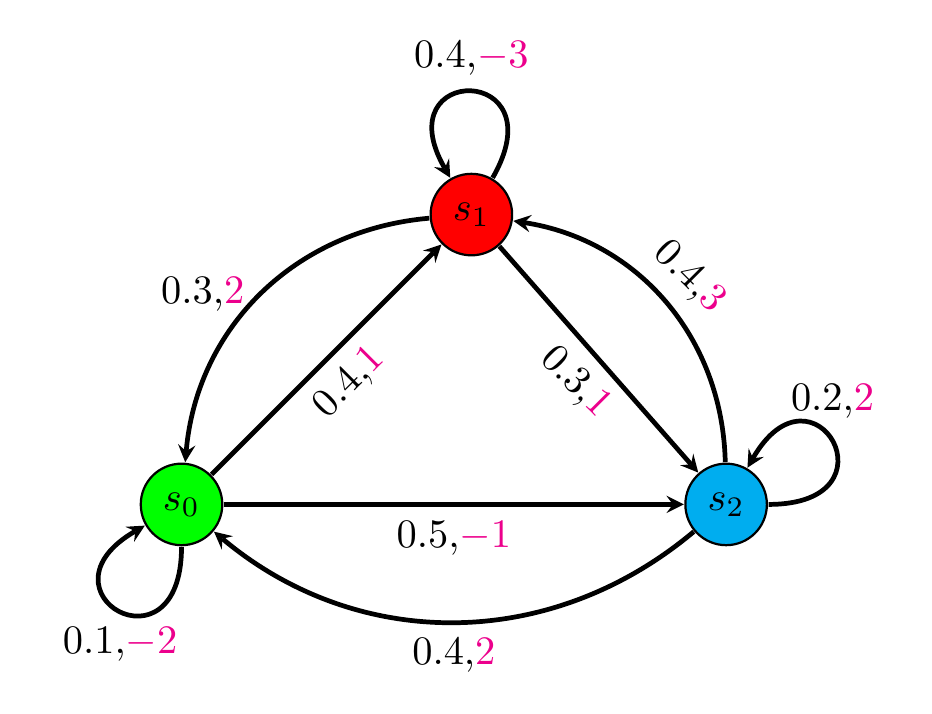
\begin{tikzpicture}[thick,scale=1.46, every node/.style={transform shape}, line width=0.6mm]
		\tikzstyle{round}=[thick,draw=black,circle]
		\node[round, fill=green] (s0) {$s_0$};
		\node[round,above right=20mm and 20mm of s0, fill=red] (s1) {$s_1$};
		\node[round, right=40mm of s0, fill=cyan] (s2) {$s_2$};
		\draw[-stealth] (s0) -- node[below, rotate=45]
		{\color{black} $0.4$\color{black},\color{magenta} $1$} (s1);
		\draw[-stealth] (s0) -- node[below]
		{\color{black} $0.5$,\color{magenta} $-1$} (s2);
		\draw[-stealth] (s1) [bend right=40] to node[left]
		{\color{black} $0.3$\color{black},\color{magenta} $2$}(s0) ;
		\draw[-stealth] (s1) -- node[below, rotate=-45]
		{\color{black} $0.3$\color{black},\color{magenta} $1$} (s2) ;
		\draw[-stealth] (s2) [bend left=40]  to node[below]
		{\color{black} $0.4$\color{black},\color{magenta} $2$} (s0);
		\draw[-stealth] (s2) [bend right=40] to node[above, rotate=-45]
		{\color{black} $0.4$\color{black},\color{magenta} $3$} (s1);
		\draw[-stealth] (s0) [out=-90,in=-150,loop] to node[below]
		{\color{black} $0.1$\color{black},\color{magenta} $-2$} (s0) ;
		\draw[-stealth] (s1) [out=60,in=120,loop] to node[above]
		{\color{black} $0.4$\color{black},\color{magenta} $-3$}(s1);
		\draw[-stealth] (s2) [out=0,in=60,loop] to node[above=2pt]
		{\color{black} $0.2$\color{black},\color{magenta} $2$}(s2);
	\end{tikzpicture}
	\caption[MDP Graph]{Markov decision process graph, transition probability is black and reward is in magenta.}
	\label{fig:mdpgraph}
\end{figure}
\\
The interaction between agent and environment can be defined by time, a discrete step implies to view it as distinct separate points in time uniquely definied and with a single state value can associated.
The sequence of observation over times form a chain of states that is called \textbf{history}, this will be particularly important because it will be used later to define the transition probability in order to model the interaction with environment.To include the reward element of an \acrshort{mdp} accumulated from present and future a new quantity need to be defined called \textbf{return}:
\begin{equation}\label{return}
	G_t = R_{t+1} + \gamma R_{t+2} + \dots = \sum_{k=0}^{\infty} \gamma^{k} R_{t+k}
\end{equation}
The $\gamma$ is a variable called discount factor with values limited inside the range of 0 and 1 with extremes included, i.e. $\gamma \in [0,1]$. The purpose of this variable is to limit the horizon of \textbf{return}, in case $\gamma$ is equal to 0 only the immediate reward will be counted and when it is 1 infinite future steps will be considered.\\
Usually the literature use $\gamma \in [0.9, 0.999]$ in order to gradually consider less relevant further time steps rewards thanks to the k-power of $\gamma$ inside \ref{return}.
The RL learning approach has the objective to maximize the \textbf{return} quantity, but this equation is not useful for the agent due to the fact that it considers every possible chain that can be observed using the Markov reward process. This means that it can vary widely even for the same state however by calculating the expectation of return from any state and  averaging a large number of chains, a new quantity can be obtained called \textbf{value of state}:
\begin{equation}
	V(s) = \mathbb{E}[G | S_t = s] = \mathbb{E}[\sum_{t=0}^{\infty} r_t \gamma^t]
\end{equation}
These formulas considers the reward and state but they are not sufficient to model environment and agent, so it is necessary to define a set of rules to control the agent behaviour considering that the objective of RL that is to maximize the return, for these reasons a new quantity must be defined \textbf{policy}.This is formally determined as probability distribution over actions for every possible state, i.e.:
\begin{equation}\label{policy}
	\pi(a|s) = P[A_t = a | S_t = s]
\end{equation}
The policy is defined as a probability in order to introduce randomness of the agent that will be useful during the training phase, if policy is fixed the transition and reward matrixes can be reduced using policy's probabilities and decreasing the action dimension.
\subsubsection{Q-learning}
As stated before the objective of RL is to maximize the return, problem is how to approximate the best optimal policy and values state in order to define the correct actions for given state. Fortunately the \textbf{Bellman optimality equation} is able to estimate approximately the best action to take on deterministic and statistical case.The equation for a general case is defined as:
\begin{equation}\label{bellman}
	V(s) = \max_{a \in A} \mathbb{E}_{s' \sim S}[(s,a) + \gamma V(s')] = \max_{a \in A} \sum_{s' \in S} p_{a, s \to s'}(r(s,a) + \gamma V(s'))
\end{equation}
The interpretation of this formula is that the optimal value state is equal to the action which gives the maximum possible expected immediate reward, plus the discounted long-term return of next state. This definition is recursive because the value state is determined from values of immediate reachable states. The formula not only gives the best reward that can be obtained, but it even gives the best policy to obtain that reward.
Formally the policy($\pi$) can now be defined as:
\begin{equation}\label{policy q learning}
	\pi(a | s) = \max_{a \in A} Q(s,a)
\end{equation}
In order to simplify this formula it is possible to define other quantities, such as \textbf{value of action}:
\begin{equation}\label{action value}
	Q(s,a) = \mathbb{E}_{s' \sim S}[r(s,a)+ \gamma V(s')] = \sum_{s' \in S} p_{a, s \to s'}(r(s,a) + \gamma V(s'))
\end{equation}
This quantity allows to define a pair of state and action, this is particulary important because it defines a category of learning called \textbf{Q-learning} which will be the focus of this thesis. As you can see using this new definition \ref{bellman} becomes:
\begin{equation*}
	V(s) = \max_{a \in A} Q(s,a)
\end{equation*}
Thanks to this, the \ref{action value} can be even defined recursively and will be particulary useful later for the deep learning approach:
\begin{equation}\label{recursive}
	Q(s,a) = r(s,a) + \gamma \max_{a \in A} Q(s',a')
\end{equation} 
The problem is that in many situations we don't know how the value of actions, rewards, transition probabilities.Due to this it the following \textbf{Q-learning algorithm} has been created:
\begin{algorithm} \label{Q-learning algo}
	\caption{Q-learning}
	\begin{algorithmic}
		\REQUIRE Discount factor($\gamma \in [0,1]$)
		\REQUIRE Memory table of dimension $N$ containing tuple: state($s$),action($a$), next state($s'$), reward($r(s,s')$) and action value $Q(s,a)$
		\STATE $i \leftarrow 0$ 
		\FOR{$i < N$}
			\STATE Apply random action $a$
			\STATE Store $(s,a,s',r)$ on memory table
			\STATE Store $Q(s,a)$ with random value
			\STATE $i \leftarrow i+1$
		\ENDFOR
		\WHILE {Until goal is reached}
			\STATE Observe current state of sistem $s$
			\STATE Define $c(s, s')$ as counter of how many times action $a$ was taken from state $s$ to transition to state $s'$
			\STATE Calculate $p(s,s') = c(s,s')/ \sum_{s' \in S} c(s,s')$
			\STATE Calculate $Q(s,a) = $ $\sum_{s' \in S}p(s,s')*( r(s,s') + \gamma\,max_{a} Q(s',a))$
			\STATE Store $Q(s,a)$ inside memory table
			\STATE Select action $a$ from policy $\pi(s|a) = max_{a} Q(s,a))$
			\STATE Apply action $a$
		\ENDWHILE
	\end{algorithmic}
\end{algorithm}\\

This Tabular Q-learning present major drawbacks such as:
\begin{itemize}
	\item A large memory table is required to store all the values used to approximate the $Q(s,a)$ values that will be used for the $\pi(s|a)$
	\item  Complete iteration over all possible states is required in order to extract the values that will be stored inside the memory table
\end{itemize} 
In order to resolve these drawbacks a new type of Q-learning algorithm called \textbf{Tabular Q-learning} was invented. The main difference is the lack of necessity to iterate over all the states to optimize because only the ones obtained from the environment will be used for optimization. Futhermore the table will only contain the $Q(s,a)$, this does not unfortunately resolve completely the drawback to have a large memory table, but at least reduce it.
\begin{algorithm} \label{Tabular Q-learning}
	\caption{Tabular Q-learning}
	\begin{algorithmic}
		\REQUIRE Discount factor $\gamma \in [0,1]$
		\REQUIRE Learning rate  $\alpha \in  [0,1]$
		\REQUIRE Memory table of dimension $N$ containing action value $Q(s,a)$
		\LOOP
			\STATE Create a table with initial values for $Q(s,a)$  
			\STATE Select random action $a$
			\STATE Observe the tuple $(s,a,r,s')$
			\STATE Calculate $V(s') = \max_{a' \in A} Q(s',a')$
			\STATE Update $Q(s,a) \leftarrow (1-\alpha) Q(s,a) + \alpha (r + \gamma V(s'))$
			\STATE Store $Q(s,a)$ inside table
			\STATE Test episode using $\pi(a|s) = \max_{a \in A} Q(s,a)$ with $Q(s,a)$ of stored values 
			\IF {goal is reached}
				\STATE break loop
			\ENDIF
		\ENDLOOP
	\end{algorithmic}
\end{algorithm}\\

As noted, a memory table is required but only to store the $Q(s,a)$ values and it will be used to update itself and to define which action need to be taken following the policy.
There is still one major problem though, this algorithm will struggle if there is a large count of the observables state set. This, in many real life situation, is quite common for example on the Cartpole environment of OpenAI gym that we are going to use there are only 4 states, but the interval of values that can be taken is enormous.
A solution of this problem would be to use a non-linear representation of action and state into a value. This is a typical "regression problem" in the field of machine learning and thanks to the power of \acrfull{nn} it is possible to approximate any kind of linear or non-linear function given enough data. Fortunately the amount of data is almost limitless thanks to the fact that if new data is needed, the only requirement is to interact more with the given environment.So now, it will be introduced the \textbf{Deep Q-learning} algorithm.

\subsection{Deep reinforcement learning}
Deep reinforcement learning is an extension of the classic one due to the use of Deep Learning techniques such as the \acrfull{nn}. Neural Networks has been introduce by \cite{Rosenblatt1958ThePA} who largely inspired by the biological brain with neurons and connections. At that time many limitations were observed due to the single layer architecture and small amount of neurons that the hardware was able to simulate, only thanks to the backpropagation algorithm introduced in \cite{backpropagation} it was later possible to train neural networks with more layers and neurons. Furthermore as demonstrated by \cite{universals} a neural network with only one single hidden layer is able to approximate any kind of linear or non-linear function, but the paper doesn't tell how many neurons are required. 
Even if the algorithms were introduced in the last century only in the last two decades thanks to hardware advancements such as GPUs and large amount of datas from the first databases it was possible to train effeciently these neural networks.
Fortunately reinforcement learning can increase the amount of data by increasing the time of interaction with the environment, but the question on how many neurons a neural networks requires to approximate doesn't have a solution, but only indications.
Now that the neural networks have been briefly introduced it is time to introduce the variation of Tabular Q-learning(\ref{Tabular Q-learning}) that uses neural networks to solve the environment.
\subsubsection{Deep Q-learning}
Tabular Q-learning is able to solve the problem of iteration over time, but it still struggles with situations when the count of observable state set is very large. This is a typical situation in real life where the set of states can be even infinite, solutions have been proposed such as use bins to discretize, but in many cases it did not result successful.
A better solution is to create a nonlinear representation, instead of a linear one, that maps both state and action to a value. This is commonly called in machine and deep learning as "regression problem" and in general does not require neural networks, but this approach is the most popular one.
Generally the following point are required to train a neural network to solve an environment:
\begin{enumerate}
	\item Initialize $Q(s,a)$ with some initial approximation.
	\item Interact with the environment to obtain tuple $(s,a,r,s')$.
	\item Calculate loss, if episode ended is $\mathcal{L} = (Q(s,a) - r)^2$ otherwise is $\mathcal{L} = (Q(s,a) - (r + \gamma \max_{a' \in A} Q(s',a')))^2$. The loss can be defined in other ways but it needs to have a difference between value of actions from current state and the discounted reward or only reward if episode ended.
	\item Update $Q(s,a)$ using an optimizer algorithm to minimize loss.
	\item Repeat from step 2 until convergence or goal reached.
\end{enumerate}

Even if it looks simple, some modifications are required in other to ensure convergence.
First of all when it is necessary to store the experience we need to find a strategy to explore the environment and optimize the current approximation, this is often referred to "exploration versus exploitation". In order to have an efficient solution it is good to behave randomly at the beginning because Q-value approximation is bad at that time and later start to act using the Q-value obtained. Usually it is used the \textbf{epsilon-greedy method} where a random probability value is sampled from a uniform distribution and confronted with a probability $\epsilon$  that tells the algorithm to behave randomly. $\epsilon$ is usually initialized to 1 so that any kind of random value sampled is smaller to $\epsilon$ so that the model behave randomly and later $\epsilon$ is decreased to a final small value so that the model will not always behave randomly but use the Q-values approximated. 
After that this problem is solved, there is another matter linked to how an optimizer algorithm work on a \acrshort{nn}. The gradients calculated from input data requires that the data are \acrshort{iid}, otherwise there would be incorrect estimations of the correct direction on which the parameters must be updated. Furthermore the data must not be completely randomic but must reflect the past actions taken in order to have an experience that tells which action are worst than others. To solve this, it is necessary to create a \textbf{large memory buffer} in order to store the past actions taken both randomic and by exploiting the agent.
Last problem that needs to be addressed is due to the steps correlation, when we calculate the loss we use $Q(s,a)$ and $Q(s',a')$ using the same \acrshort{nn}, this can be a problem because $s$ and $s'$ are highly correlated and this can lead to similar approximation. This influence the convergence of learning during the training process, to deal with it a copy of the \acrshort{nn} is created and updated by copying parameters of the original one with a fixed interval, this \acrshort{nn} is usually called \textit{target network}.
The following pseudo is taken from the original paper that was tested on atari games \cite{DBLP:journals/corr/MnihKSGAWR13}, after this paper numerous variations have been proposed in order to improve convergence and reduce time of training, such as Double Q-Net \cite{DBLP:journals/corr/HasseltGS15} and many others. Due to the limited resources and time required the thesis will be focused on the "classical" DQN, but it would be interesting to verify if the advantage would be more pronounced or reduced.
\begin{algorithm} \label{DQN}
	\caption{Deep Q-Networks}
	\begin{algorithmic}
	\REQUIRE Memory buffer of dimension $N$ containing tuple: state($s$),action($a$), next state($s'$), reward($r(s,s')$)
	\REQUIRE Discount factor $\gamma \in [0,1]$
	\REQUIRE Learning rate  $\alpha \in  [0,1]$
	\REQUIRE Optimizer
	\REQUIRE A neural networks for $Q$ and target network for $\hat{Q}$
	\REQUIRE $\epsilon$ probability of randomness
	\STATE Initialize $Q(s,a)$ and $\hat{Q}(s,a)$ with random weights and empty memory buffer, $\epsilon \leftarrow 1.0$
	\WHILE {goal not reached}
	\STATE Observe state and define with probability $\epsilon$ if $a$ is random or $a = \arg \max_{a \in A} Q(s,a)$
	\STATE Apply $a$, observe $r$ and $s'$, store in memory buffer the tuple $(s,a,r,s')$
	\STATE Sample a batch of tuple $(s,a,r,s')$
	\STATE For every tuple calculate $y = r$ if episode ended for that state, otherwise calculate $y = r + \gamma \max_{a' \in A} \hat{Q}(s',a')$
	\STATE Calculate loss $\mathcal{L} = (Q(s,a) - y)^2$
	\STATE Use optimizer to update $Q(s,a)$ parameters in order to minimize $\mathcal{L}$ 
	\STATE Every $n$ steps copy weights of $Q$ to $\hat{Q}$
	\ENDWHILE		
	\end{algorithmic}
\end{algorithm}\\

The \ref{DQN} gave a breakthrough on this field thanks to the fact that was able to achieve a human-like, and in some cases even better, performance on multiple games of the atari. Thanks to this \acrlong{drl} has been tested and applied in other contexts such as finance, medicine, robotics and many others. Before we introduce quantum computing it is necessary to explain and describe another algorithm that is able to handle \acrlong{mdp} without the value iteration method: \textbf{policy gradient methods}.
\subsubsection{Policy gradient methods}
The \acrshort{dqn} that we have illustrated is focusing mainly on approximating the value of actions($Q$) and the value of state($V$) so that afterward the choice on which action to take is based on a greedy approach: the best action to take is the one that maximize the return. This is not incorrect, but in some cases it may not be good due to the environment consequences. For this reason in those cases it is better to focus on how to define the agent behaviour in order to consider vene the possible alternatives. Another reason why these methods are used is due to the fact that can introduce \textbf{stochasticity} and can work on \textbf{continous environment} differently from the \acrshort{dqn} showed.
Now that the method is focused on policy, it is necessary to give a \textbf{policy representation} in order to work with it, the most common way is to use a probability distribution over the possible actions. This gives an additional advantage to neural network which is to have a smooth representation, in other words if a variation is applied on the weights outputs variate.
It is now time for the final step, to find a way to optimize the weights in order to improve the policy. Thanks to the policy gradient theorem, it is known that the formula we need to use is:
\begin{equation}\label{policy_grad_theorem}
	\nabla J \approx \mathbb{E}[Q(s,a) \nabla \log \pi(a|s)]
\end{equation}
the complete demonstration of the formula and application on \acrlong{drl} can be found on \cite{10.5555/3009657.3009806}. The meaning of this expression can be as follow: the policy gradient tells us the direction of update, the formula is proportional to the value of action taken $Q(s,a)$ and the gradient of log probability action taken. Simply we are trying to increase the probabilty of good actions and rewards, at the same time decreasing the probability of bad actions and outcomes. Finally, the $\mathbb{E}$ is expectation value due to the fact that will be used with multiple values.
There are some drawbacks for this approach such as a high gradients variance that can influence the learning and exploration at the beginning of training and to avoid falling in a local minima it is necessary to introduce some kind of uncertainty or \textit{entropy}. There is another problem of policy gradient methods and that is the fact that are usually less sample-efficient and this implies a bigger numeber of iterations to solve the environment. In order to tackle this problems new algorithms have been defined, notably \acrfull{a2c} [\cite{DBLP:journals/corr/WangBHMMKF16}], \acrfull{ppo}[\cite{DBLP:journals/corr/SchulmanWDRK17}] and others which tries to reap the benefits of policy and value methods. This thesis will use the \acrfull{sac} algorithm on a robotic environment and later will confront it with the quantum type.
\subsubsection{Soft Actor Critic}
This algorithm can be seen as a variation of Actor-Critic, the latter one can be simplified as the necessity to improve the behaviour and values of states approximated in order to solve the environment. In order to achieve this two neural networks are used: one to approximate the policy called \textbf{policy net or actor} and one to approximate the value of state called \textbf{value net or critic}.
\begin{figure}[!ht]
	\centering 
	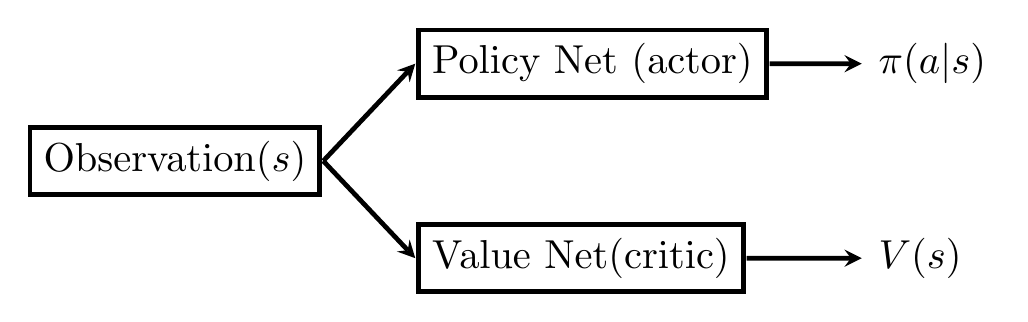
\begin{tikzpicture}[thick,scale=1.46, every node/.style={transform shape}, line width=0.6mm]
		\node[rectangle, draw] (obs) {Observation($s$)};
		\node[rectangle, draw, above right=2mm and 8mm of obs] (policy) {Policy Net (actor)};
		\node[rectangle, draw, below right=2mm and 8mm of obs] (value) {Value Net(critic)};
		\node[right=8mm of policy] (pi) {$\pi(a|s)$};
		\node[right=10mm of value] (v) {$V(s)$};
		\draw[-stealth] (obs.east) -- (policy.west);
		\draw[-stealth] (obs.east) -- (value.west);
		\draw[-stealth] (policy.east) -- (pi.west);
		\draw[-stealth] (value.east) -- (v.west);
	\end{tikzpicture}
	\caption[a2cflow]{Schematic on actor-critic architeture}
	\label{fig:a2cflow}
\end{figure}
The problems of this algorithm is the fact that is on-policy and sensible to hyperparameters, in order to improve performance, stability and efficiency the \acrshort{sac} was created.
\acrshort{sac} is able to do it introducing multiple components such as : 
\begin{itemize}
	\item a large buffer memory is needed to efficiently update the weights using previous history increasing in this way stability and switching to an off-policy method instead of an on-policy one.
	\item A target network of the critic net is introduced to improve the stability and efficiency of learning to approximate the value state, differently from the \acrshort{dqn} updating target network will follow the procedure of \textbf{soft functions update}. Shortly, this means that the values will use a factor to combine new and old weights obtained from the update step, to do this a loss value of state ($J_{V}$) and action ($J_{Q}$) function must be defined.
	\begin{equation}\label{state of calue loss}
		J_{V}(\psi)= \mathbb{E}_{s \sim S}\left[ \frac{1}{2} (V_\psi(s_t) - \mathbb{E}_{a_t \sim \pi_\phi}[Q_\theta(s_t,a_t) - \log \pi_{\phi}(a_t|s_t)])^2 \right]
	\end{equation}
	\begin{equation}\label{state of action loss}
		J_{Q}(\theta)= \mathbb{E}_{s \sim S, a \sim A }\left[\frac{1}{2}(Q_\theta(s_t,a_t) - r(s_t,a_t) + \gamma \mathbb{E}_{s_{t+1} \sim p}[V_{\overline{\psi}}(s_{t+1})] )^2 \right]
	\end{equation}
	\item the maximum entropy of reinforcement learning is introduced to increase the exploration of environment, improve learning and reduce sensibility to hyperparameters.The loss of this maximum entropy was transformed for this case from the "classical" one considering the use of a neural network and introducing an input noise vector($\epsilon_t$) sampled from the a fixed spherical gaussian distribution to calculate the action.\\
	Output action of neural network and input noise from currrent state can be expressed as follows $a_t = f_\phi(\epsilon_t;s_t)$ bringing to the loss formula:
	\begin{equation}\label{policy loss}
		J_{\pi}(\phi)= \mathbb{E}_{s \sim S, \epsilon_t \sim \mathcal{N}}\left[ \log \pi_{\phi}(f_\phi(\epsilon_t;s_t)) - Q_{\theta}(s_t, f_\phi(\epsilon_t;s_t))\right]
	\end{equation}
\end{itemize}
For more details on how these formulas have been obtained and experimental results refer to the original paper \cite{DBLP:journals/corr/abs-1801-01290}, to avoid confusion the pseudocode will be showed later considering that there are variations from the original implementation to create a quantum version, so that later it would be possible to confront classical and quantum algorithm.
\subsection{Quantum computing}
Quantum computing is a field that originated around the 1980s by numerous physicists, Paul Benioff was first to introduce the idea of a Turing machine that used quantum mechanics to make calculation. Richard Feynman and Yuri Manin suggested to use it for efficient simulation on quantum mechanics systems. Futhermore David Deutsch asked if using physical laws it was possible to derive a stronger version of the Church-Turing thesis introducing the concept of Universal Quantum Computing, this conjecture isn't still demonstrated but has paved the way for current concept. In order to introduce quantum computing it is necessary to understand what is a quantum bit, circuit and logic gate, keeping in mind that even if the following representation is an abstraction there is a physical implementation for all this components.
\subsubsection{Quantum bits}
Quantum bits or qubits are the analogous of classical bits which are used as a fundamental concept for computation and information forming a computational bases states. As the bits can have two possible states 0 and 1, the qubits, thanks to the discretized energy on a microscopic level, can have a quantum state $\ket{0}$ and $\ket{1}$. Differently from their classical counterparts and thanks to the quantum mechanics, the qubits can be in a possible \textit{linear combination} even known as \textit{superposition} of states:
\begin{equation}\label{superposition}
	\ket{\psi} = \alpha \ket{0} + \beta \ket{1}
\end{equation}
The numbers $\alpha$ and $\beta$ are complex even known as \textit{amplitudes}, so a qubit can be represented as a two-dimensional complex vector space. A fundamental condition is applied on these numbers to respect the statistical view of quantum mechanics, when a qubit is measured a probability of being on the quantum state is associated. These probabilities can be represented as $|\alpha|^2$ to be in state $\ket{0}$ and $|\beta|^2$ in state $\ket{1}$, for natural statistic normalization these number must have the condition $|\alpha|^2 + |\beta|^2 = 1$.Geometrically this can be interpreted as the fact that qubit states must be normalized in order to have length 1 and be rewritten using real numbers as:
\begin{equation}
	\ket{\psi} = e^{i\gamma} \bigg( \cos{\frac{\theta}{2}} \ket{0} + e^{i\varphi} \sin{\frac{\theta}{2}} \ket{1}\bigg)
\end{equation}
with $\gamma, \theta, \varphi \in R$. Due to the fact that there are no observables effects with a global phase, it is possible to ignore $e^{i\gamma}$ giving the reduced formula:
\begin{equation}\label{angle qubits}
	\ket{\psi} = \cos{\frac{\theta}{2}} \ket{0} + e^{i\varphi} \sin{\frac{\theta}{2}} \ket{1}
\end{equation}
This allows to introduce a three-dimensional sphere representation called \textbf{Bloch sphere} showed in figure \ref{bloch sphere}, which allows to represented any possible superposition of states in a qubit.
\begin{figure}[!ht]
	\centering
	\scalebox{1.8}{
	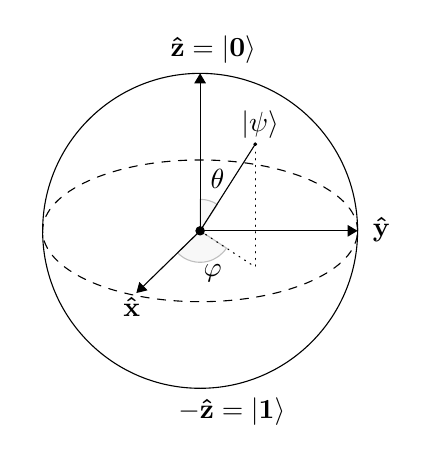
\begin{tikzpicture}[line cap=round, line join=round, >=Triangle]
		\clip(-2.19,-2.49) rectangle (2.66,2.58);
		\draw [shift={(0,0)}, lightgray, fill, fill opacity=0.1] (0,0) -- (56.7:0.4) arc (56.7:90.:0.4) -- cycle;
		\draw [shift={(0,0)}, lightgray, fill, fill opacity=0.1] (0,0) -- (-135.7:0.4) arc (-135.7:-33.2:0.4) -- cycle;
		\draw(0,0) circle (2cm);
		\draw [rotate around={0.:(0.,0.)},dash pattern=on 3pt off 3pt] (0,0) ellipse (2cm and 0.9cm);
		\draw (0,0)-- (0.70,1.10);
		\draw [->] (0,0) -- (0,2);
		\draw [->] (0,0) -- (-0.81,-0.79);
		\draw [->] (0,0) -- (2,0);
		\draw [dotted] (0.7,1)-- (0.7,-0.46);
		\draw [dotted] (0,0)-- (0.7,-0.46);
		\draw (-0.08,-0.3) node[anchor=north west] {$\varphi$};
		\draw (0.01,0.9) node[anchor=north west] {$\theta$};
		\draw (-1.10,-0.72) node[anchor=north west] {$\mathbf {\hat{x}}$};
		\draw (2.07,0.3) node[anchor=north west] {$\mathbf {\hat{y}}$};
		\draw (-0.5,2.6) node[anchor=north west] {$\mathbf {\hat{z}=|0\rangle}$};
		\draw (-0.4,-2) node[anchor=north west] {$-\mathbf {\hat{z}=|1\rangle}$};
		\draw (0.4,1.65) node[anchor=north west] {$\ket{\psi}$};
		\scriptsize
		\draw [fill] (0,0) circle (1.5pt);
		\draw [fill] (0.7,1.1) circle (0.5pt);
	\end{tikzpicture}
	}
	\caption[The bloch sphere]{Representation of a qubit the Bloch sphere}
	\label{bloch sphere}
\end{figure}

This formalism can be extended  for the case of multiple qubits, if for example a system is composed of two separable qubits $\ket{\psi}$ and $\ket{\phi}$ then it is possible to construct their representation $\ket{\nu}$ using the dot product as follows:
\begin{align*}
	\ket{\psi} &= \alpha \ket{0} + \beta \ket{1} \qquad
	\ket{\phi} = \gamma \ket{0} + \delta \ket{1}\\
	\ket{\nu} &= \ket{\psi} \otimes \ket{\phi} = \alpha\gamma \ket{00} + \alpha\delta \ket{01} + \beta\gamma \ket{10} + \beta\delta\ket{11}\\
\end{align*}
The previous form of $\ket{00}$ is only an abbreviation for the form $\ket{0} \otimes \ket{0}$,
normalization must be still valid so the sum of all amplitudes squared must give 1, in other words $|\alpha\gamma|^2  + |\alpha\delta|^2  + |\beta\gamma|^2  + |\beta\delta|^2 = 1$ if that is not the case it is possible to normalize it dividing by the root square of the squared sum. As it can be seen with only two qubits there are four quantum states, if for example we had $N$ qubits then there would be $2^N$ possible states giving a tremendous advantage on the information that can be stored instead of the classical approach.
Furthermore thanks to the fact that this is a multi dimensional space a matrix representation to give the following formalism:
\begin{align*}
	\ket{0} =   
		\begin{bmatrix}
			1 \\
			0
		\end{bmatrix}
	\qquad
	\ket{1} &=
	   \begin{bmatrix}
	   	0 \\
	   	1
	   \end{bmatrix}
    \qquad
    \ket{\psi} =
   		\begin{bmatrix}
   		 \alpha \\
   		 \beta
   		\end{bmatrix}
   	\qquad
   	\ket{\phi} =
   		\begin{bmatrix}
   		\gamma \\
   		\delta
   		\end{bmatrix}\\
   		\ket{\nu} &= \ket{\psi} \otimes \ket{\phi} = 
   		\begin{bmatrix}
   			\alpha\gamma & \alpha\delta\\
   			\beta\gamma  & \beta\delta
   		\end{bmatrix}\\
\end{align*}
In case a measurement is applied on subsets of qubits, for example on the first qubit measuring if the state is $\ket{0}$ then the post-measurement state will be:
\begin{equation}\label{post measurement}
		\ket{\nu'} = \frac{\alpha\gamma\ket{00} + \alpha\delta \ket{01}}{\sqrt{|\alpha\gamma|^2 + |\alpha\delta|^2}}
\end{equation}
the denominator is due to normalization after measurement in order to respect the condition that squared amplitudes summed is 1.\\
Quantum mechanics allows even some particular states called \textit{Bell states or EPR pair} which are not separable such as this one:
\begin{equation}\label{bell state}
	\frac{\ket{00} + \ket{11}}{\sqrt{2}}
\end{equation}
even if it seems to be completely normal, notice that in case a measurement is applied on any of the two qubits it is possible to know immediately with certainity what state is in the other one. So there is a \textit{correlation} between the qubits, point is that this type of correlation is \textbf{stronger than any kind that could exist classicaly}. This correlation is known as \textbf{entanglement}, is at the basis of many quantum algorithms and has been proven to be valid even on distance of galaxies. This doesn't violate Einstein general relativity because the information even if using this quantum property in any case can't exceed the speed of light. Now that the separated and entangled states have been introduced it is time to see how the qubits can be manipulated using the \textbf{gates and circuits}.
\subsubsection{Quantum gates and circuits}
As classical computation uses \textit{wires} amd \textit{logic gates}, quantum computing does the same. Main difference is that for example quantum gates such as the equivalent quantistic NOT act linearly instead of non-linearly, the reason is due to the fact that if non-linearity was allowed then empirically there would be paradoxes, such as violations of the second law of thermodynamics, faster than light communications and time travels. Taking advantage of the linear proprierty it is possible to give a matrix form of such as NOT, in fact a NOT gate classicaly invert 0 to 1, what happens on quantum computing is:
\begin{equation*}
	\alpha \ket{0} + \beta \ket{1} \to \beta \ket{0} + \alpha \ket{1}
\end{equation*}
in matrix form it can be translated as:
\begin{equation*}
	X = \begin{bmatrix}
		0 & 1 \\
		1 & 0
	\end{bmatrix}
	\to
	X \begin{bmatrix}
		\alpha \\
		\beta
	\end{bmatrix}
	= \begin{bmatrix}
		\beta \\
		\alpha
	\end{bmatrix}
\end{equation*}
In addition to the linearity of quantum gates, it is necessary to remember that these operations must respect the condition of normalization equal to 1. This can be translated to the condition that any matrix $U$ representing a quantum gate, must be unitary. This can be formalized using the \textit{adjoint} of $U^\dag$, which means complex conjugating and transposing the elements of U, as the condition $U^\dag U = 1$. This can be even interpreted as the fact that any kind of quantum operation applied is reversible, so by applying another one is possible to return at the initial state, which quantistically is the adjoint of operation applied.
The most used single qubit gates are the following:
\begin{equation*}
	X = \begin{bmatrix}
		0 & 1 \\
		1 & 0 
	\end{bmatrix}\qquad
	Y = \begin{bmatrix}
		0 & -i \\
		i & 0
	\end{bmatrix}\qquad
	Z = \begin{bmatrix}
		1 & 0 \\
		0 & -1 
	\end{bmatrix}
	H = \frac{1}{\sqrt{2}}\begin{bmatrix}
		1 & 1 \\
		1 & -1
	\end{bmatrix}
\end{equation*}
there are other gatex such as S, T and I, for the thesis they will not be necessary, but if interested feel free to check the book(put reference Nielsen Chang).The interesting part is that any kind of single qubit gate can be obtained from the generic form:
\begin{equation}\label{generic gate}
	U(\theta,  \phi, \lambda) =  \begin{bmatrix}
		\cos(\frac{\theta}{2}) & -e^{i\lambda} \sin(\frac{\theta}{2})\\
		e^{i\phi}\sin(\frac{\theta}{2}) & e^{i(\phi+ \lambda)}\cos(\frac{\theta}{2})
	\end{bmatrix}
\end{equation}
for confirmation as an example notice that $H = U(\frac{\pi}{2}, 0, \pi)$.\\
Now as there a single qubit gates, it is possible to extend the concept introducing \textbf{multiple qubit gates}. These, differently from the single qubits using multiple of them, for example one that will be used extensively is the \textit{controlled-NOT} or CNOT gate which has the following form:\\
\begin{center}
	\begin{quantikz}[scale = 3.0]
		 &  \ctrl{1} & \qw\\
		 &  \targ{}  & \qw
	\end{quantikz}
\end{center}
\begin{equation*}
	CNOT = 
	\begin{bmatrix}
		1 & 0 & 0 & 0 \\
		0 & 1 & 0 & 0 \\
		0 & 0 & 0 & 1 \\
		0 & 0 & 1 & 0
	\end{bmatrix}
\end{equation*} 
This gate function by using a control qubit which is the black dot and only if the control qubit is $\ket{1}$ applies to the target qubit $\oplus$ which is the addition modulo two operation that on a two basis computational state means to flip it. The horizontal line repreent the wire used to transfer the qubit. Formally CNOT is defined as:
\begin{equation*}
	\ket{00} \to \ket{00} \qquad \ket{01} \to \ket{01} \qquad \ket{10} \to \ket{11} \qquad \ket{11} \to \ket{10}
\end{equation*}
The import point is that this circuit is like it applies an $X$ gate, in fact it is possible to subsitute with other single qubit gate. There are other multi qubit gates such as \textit{toffoli}, \textit{swap} and many others, but they will not be used in this thesis.
The reason for which \textbf{CNOT is largely used because it can introduce the entanglement effect on qubits}, this is particularly important to efficiently explot the quantum advantage. For example the \ref{bell state} can be obtained with the following circuit:
\begin{center}
	\begin{quantikz}[scale = 3.0]
		\lstick{$\ket{0}$} & \gate{H} &  \ctrl{1} & \qw\\
		\lstick{$\ket{0}$} & \qw &  \targ{}  & \qw
	\end{quantikz}
\end{center}
Now that gates and wires have been introduced it is not necessary to introduce onle last component the measurement gate, in fact after the qubits are manipulated it is necessary to extract the information on these. In order to do that a measurement basis can be decided and quantum computing allows more than the classical basis of $\ket{0}$ and $\ket{1}$, but only this one will be used.As said the measurement consist of extracting information, but for the quantistic case this means distinguish the possible states, this is represented with the following symbol on circuits:
\begin{center}
	\begin{quantikz}[scale = 3.0]
		 & \meter{} & \qw
	\end{quantikz}
\end{center}
This measurement on the computational basis consist on using projectors of the possible eigenspaces, for the case of a generic qubit state projectors are $P_{0} = \ket{0} \bra{0}$ and $P_1 = \ket{1} \bra{1}$. The probability associated to be in one state, for example $\ket{0}$ can be defined as:
\begin{equation*}
	p(0) = tr(P_0 \ket{\psi}\bra{\psi}) = \bra{\psi}P_0\ket{\psi} = |\alpha_0|^2
\end{equation*}
The fully observable corresponding to a computational basis measurement is the Pauli-Z operator or the Z gate:
\begin{equation*}
	\sigma_z = \ket{0} \bra{0} - \ket{1}\bra{1} = Z
\end{equation*}
To work with quantum computing it is necessary to use statistics and in order to have the correct expectation value of $<\sigma_z>$ it is necessary to repeat multiple times the measurement to sample the possible values, his is usually represented as $S$ which is an abbreviation for \textit{shots}. In order to have the correct expectation with an error of at most $\epsilon$ conventional statistics can be used for example using the Bernoulli distribution.
Error gives a confidence interval $[p-\epsilon, p + \epsilon]$ which tells the proportion of samples that are in the interval. Statistically this can be associated to a $z$-value.
Estimating the error of a Bernoulli trial can be defined in different  ways, but the most preferred ways is by using the Wilson score interval \cite{10.2307/2276774}. Following that formula the overall error of estimation is bounded by the following equation:
\begin{equation*}
	\epsilon \le \sqrt{z^2 \frac{S +z^2}{4S^2}}
\end{equation*}
which can be inverted to calculate the S required:
\begin{equation*}
	S \le \frac{\epsilon^2 \sqrt{\frac{z^4(16\epsilon^2 + 1)}{\epsilon^4}} + z^2}{8\epsilon^2}
\end{equation*}
\subsubsection{Quantum decoherence}
There is phenomenon that needs to be considered when a quantum device is effectively used and that is \textbf{quantum decoherence}. The phenomenon is refeered to the effect of losing quantum coherence, this is obtained when the phase relation of the wave functions associated to different states is not valid anymore. This effects is mainly due to the fact that qubits are not completely isolated and interactions with environment introduce entanglement between them. The effect of quantum decoherence is problematic because implies loss of information stored.\\
This effect for quantum computing introduces non-linearity and is usually considered through quantities called \textit{decoherence times}. These are defined as $T_1$ and $T_2$, $T_1$ refers to \textit{relaxation time} which is the time taken to transition from $\ket{1} \to \ket{0}$. $T_2$ refers instead to \textit{dephasing time} that is the time for which qubits phase remains intact. These times are usually combined and used as costant decays for statistically say when quantum decoherence affect the qubits. Application of quantum gates influence the system by increasing the possibility of decoherence, for this reason \textbf{quantum error correction} has been developed. Problem is that these algorithms for error correction requires a lot of qubits and actually there are not physical devices with this capacity.\\
In order to deal with the quantum decoherence from environment and gates, new types of algorithms have been created with the requirement to use the least number of gates and operations required to successfully extract information.
\subsubsection{Encoding algorithms}
Working with quantum computers requires that information which needs to be analyzed and transformed needs to quantistic, there are different ways to encode: \textit{basis encoding, amplitude encoding, angle encoding.} There are even others in \cite{Schuld2021}, but these will be the ones used in this thesis.
Basis encoding is based on the fact that any bit is substituted with the qubit having corrisponding state value, for example $01001$ becomes $\ket{01001}$ using this strategy. As it is possible to notice this representation is not qubit efficent because it requires the same number of qubits for the associated bit of value, but the routine don't require many operations. Another strategy of encoding is called \textit{amplitude encoding}, which consist of taking the value of a classical vector $x$, normalize the values inside by normalizing the elements and associate to them an amplitude, like in this exxample:
\begin{align*}
	& x \to \sum_{k=1}^{2^n}|x_k| ^ 2 = 1 \\
	&x = \begin{bmatrix}
		x_1 \\
		\vdots \\
		x_{2^n}
	\end{bmatrix}
	 \leftrightarrow
	 \ket{x} = \sum_{j} x_j \ket{j}
\end{align*}
this kind of representation requrires very few qubits, but the routine required to encoded it is not applicable on the actual physical devices for their limited capabilities. The last strategy is the \textit{angle encoding} which consist on applying a rotation of the classical value along one axis, this is used because it can exhibit some similarities and proprierties to the amplitude encoding. It is not qubit efficient, but the routine can be applied using actual devices, formally it can be defines as follows:
\begin{equation*}
	x \to \ket{x} = \otimes_{i}^{n} R(x_i) \ket{0^i}
\end{equation*}
where $R$ can be $R_x, R_y, R_x$ so it is only necessary to apply one single rotation gate over every qubit using as angle the classical value.
%%
%%\subsection{Summary}
%%In this section it has been introduced reinforcement learning, deep reinforcement learning %%and quantum computing. It has been introduced the \acrlong{mdp} and Q-learning as basis for %%\acrlong{drl} and algorithms such as \acrlong{dqn} and \acrlong{sac} has been showed to deal %%with environments that can be discrete and continous. Futhermore it has been introduced %%quantum computing from the definition of qubits to gates and circuits. Quantum decoherence %%has been introduced such as one of the main limitations to the application of quantum %%algorithms using actual devices and encoding startegies has been explained on how to convert %%classical into quantum information. Now that introduction is finished, time has come to see %%how Quantum algorithms such as \acrfull{vqa} can be used to solve difficult environments and %%are applicable to actual \acrfull{qpu}.

	\section{Variational circuits applied to deep reinforcement learning}
Variational circuit or \textit{parametrised circuit}, are a type of quantum computing model that can be used in the field of machine learning. The problems that this model tries to tackle are: find the best parameters to solve the problem required and applicability to actual physical quantum devices with their limitations. This kind of circuit is \textit{hybrid}, because it uses concept that comes from quantum and classical algorithms, futhermore it can be applied to actual quantum devices with classical computer. The usual approach for this kind of circuit is to use quantum algorithms as the machine learning model and apply the training on data using classical algorithms. In this thesis it will be used as a layer for \acrfull{nn}, due to the fact that these kinds of circuits can be even viewed as \textit{quantum neural networks} thanks to their approximation ability to functions and because deep learning models are particularly successfull in \acrfull{rl}. A consideration that needs to be done is the fact that an ideal variational circuit must be small as possible in order to make it work on a quantum device and reduce the possibility of information loss due to decoherence, this type of circuit is referred as \textbf{shallow circuit}. An extensive paper that describes these circuit is \cite{Cerezo_2021}.
\subsection{Variational Circuit}
Variational circuits have been fromulated by \cite{https://doi.org/10.48550/arxiv.1802.06002}-\cite{Benedetti_2019}, but the idea was introduced years before. This circuit are based from the fact that gate can have an associated a parameter, the parametrized and unparametrized gates that will be used in the circuit will form an \textbf{ansatz}.In order to optimize the parametrized circuit it is necessary to define a cost function $C(\theta)$ and find an optimizer algorithm able to find the set parameters for which this cost function is minimized. This optimizer usually is based on gradient methods to reach the set of parameters that minimize the cost function, fortunately the gradient of a variational circuit can be calculated quite easily using a method called \textbf{parameter shift} as it will be seen later.\\
Thanks to the proprierties of quantum mechanics the entire circuit can be considered as a single unitary gate of the form $U(x,\theta)$ due to their dependecies on the input data. Usually the internal structure of $U(x,\theta)$ consist on of an embedding block $S(x)$ and a parametrized one $W(\theta)$ in order to decompose $U(x,\theta) = S(x)W(\theta)$, these blocks can contains quantum fixed gates. Graphycally this can be seen as:\\
\begin{center}
	\begin{figure}[!h]
		\centering
		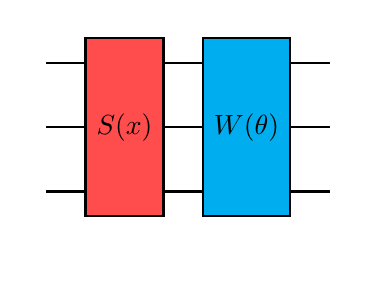
\begin{tikzpicture}
		\node{
		\begin{quantikz}
			& \gate[wires= 3, style={fill=red!70}]{S(x)} & \gate[wires = 3, style={fill=cyan}]{W(\theta)} & \qw \\
			& & & \qw \\
			& & & \qw \\
		\end{quantikz}
		};
		\end{tikzpicture}
	\caption{ususal decomposition of quantum circuit}
	\label{sw}
	\end{figure}
\end{center}
So in the end a variational circuit can be graphically summarized as follows:
\begin{center}
	\begin{figure}[!h]
	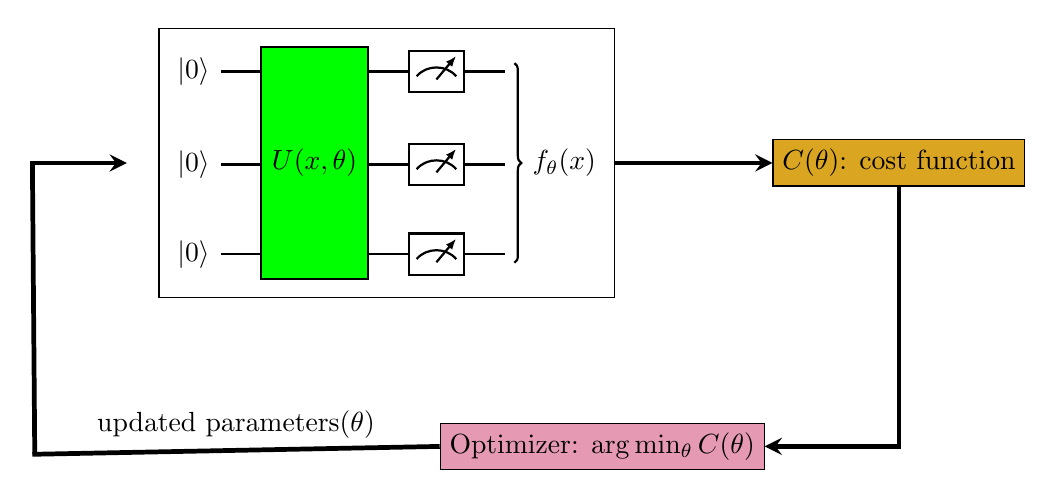
\begin{tikzpicture}
		%%nodes
		\node[draw] (qc){
		\begin{quantikz}
			\lstick{$\ket{0}$} & \gate[wires= 3, style={fill=green}]{U(x, \theta)} & 	\meter{} & \qw\rstick[wires=3]{$f_{\theta}(x)$} \\
			\lstick{$\ket{0}$}& & \meter{} & \qw \\
			\lstick{$\ket{0}$}& & \meter{} & \qw
		\end{quantikz}
		};
		\node[draw,fill=Goldenrod, right=20mm of qc] (cost) {$C(\theta)$: cost function};
		\node[draw,fill=purple!40, below left=30mm and 1 mm of cost] (opt) {Optimizer: $\arg \min_{\theta} C(\theta)$};
		\draw[-stealth, line width=0.6mm] (qc.east) -- (cost.west);
		\draw[-stealth, line width=0.6mm] (cost.south) |- (opt.east);
		\draw[line width=0.6mm] (opt.west) -- node [midway,above,align=center ] {updated parameters($\theta$)} (-4.5,-3.7);
		\draw[line width=0.6mm] (-4.47,-3.7) -- (-4.5,0);
		\draw[-stealth, line width=0.6mm] (-4.53,0) -- (-3.3,0);
	\end{tikzpicture}
	\caption{Schematic of a variational quantum algorithm} 
	\label{vqa graph}
	\end{figure}
\end{center}
Furthermore these variational circuits can be interpreted, with minor conceptual changes, to deterministic or probabilistics machine learning models and can be ingtegrated, as it will be seen in this thesis, as a component of neural networks.\\
\subsubsection{Deterministic quantum model}
\begin{mydef}
	Considering a data domain $X$, the quantum circuit $U(x, \theta)$ with $x \in X, \theta \in \mathbb{R}^n$ depends on input data and indicating $\mathcal{M}$ as an hermitian operator associated to a quantum observable. It is possible to denote $\ket{\psi{x,\theta}}$ as  $U(x,\theta)\ket{0}$ then it is possible to define the output of this variational circuit as:
	\begin{equation}\label{quantum deterministic}
		f_\theta(x) = \bra{\psi(x, \theta)} \mathcal{M}  \ket{\psi(x, \theta)} = \braket{\mathcal{M}}_{x,\theta}
	\end{equation}
\end{mydef}
This formula tells that even if quantum computing output is statistical, an average value based on the measurement applied can be extracted. For example if measurement is written in diagonal basis such as : $\mathcal{M} = \sum_i \mu_i \ket{\mu_i} \bra{\mu_i}$, then the output function will be of the form of:
\begin{equation*}
	f_\theta(x) = \sum_i \mu_i |\braket{\mu_i |\psi(x, \theta)}|^2 = \sum_i \mu_i p(\mu_i)
\end{equation*}
In case the measurement applied is based on the Z-gate($\mathcal{M} = Z$) which will be the one iused in the following variational quantum algorithm the result can be rewritten by considering the eigenvalues and eigenstates obtaining the following result:
\begin{equation*}
	f_\theta(x) = |\braket{0|\psi(x, \theta)}|^2 - |\braket{1| \psi(x, \theta)}|^2 = p(0) - p(1)
\end{equation*}
This quantity can be even calculated by performing $S$ shots sampling the eigenvalues $\mu^(s) \in {\mu_i}$ and averaging over the results, obtaining the following form:
\begin{equation*}
	\hat{f}(x) = \frac{\sum_{i=1}^{S}\mu_i}{S}
\end{equation*}
This value can be estimated with an error $\epsilon$ applying $O(\epsilon^{-2})$ measurement, this means that if for example the error required is 0.01, then the measurement needed to be applied is of the order in 1000s. This deterministic function will be used mainly for approximating the q-value and other quantity necessary for the reinforcement learning algorithm. 
\subsubsection{Probabilistic quantum model}
The inherit theory of quantum mechanics allows for these models to be expressed as probabilistic, in fact as it will be seen later \acrfull{vqa} can be interpreted as supervised and unsupervised model applying minimal modifications on the quantum circuit.
\begin{mydef}[supervised probabilistic quantum model]
	Let $X$ be an input and $Y$ an output domain, and $U(x, \theta)$ be an input and parameter-
	dependent unitary so that $\psi(x, \theta) = U(x, \theta)\ket{0}$. We associate each eigenvalue	or outcome of a measurement observable with a possible output $y$, so that $\mathcal{M} \sum_{y \in Y} y \ket{y} \bra{y}$. A supervised probabilistic quantum model for a conditional distribution is then defined:
	\begin{equation}
		p_\theta(y|x) = |\braket{y|\psi(x, \theta)}|^2
	\end{equation}
\end{mydef}
Due to ${\ket{y}}$ being a basis, the normalization is required so $\sum_{y \in Y} \ket{y} \bra{y} = \mathbbm{1}$ and probability sum to 1.Representing this kind of variational quantum circuit using the previous ansatz, it can be represented as:
\begin{center}
	\begin{figure}[!h]
		\centering
		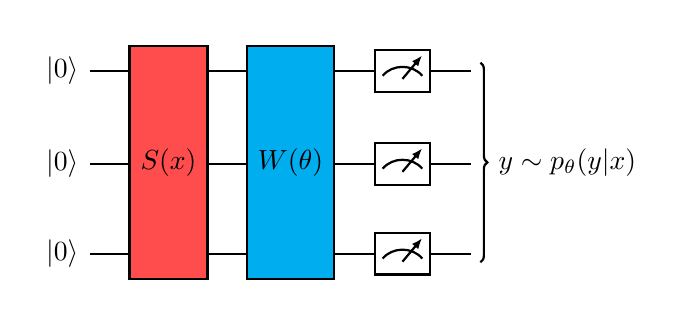
\begin{tikzpicture}
			\node{
				\begin{quantikz}
					\lstick{$\ket{0}$} & \gate[wires= 3, style={fill=red!70}]{S(x)} & \gate[wires = 3, style={fill=cyan}]{W(\theta)} & \meter{} & \qw\rstick[wires=3]{$y \sim p_\theta (y|x)$} \\
					\lstick{$\ket{0}$}& & & \meter{} & \qw \\
					\lstick{$\ket{0}$}& & & \meter{} & \qw
				\end{quantikz}
			};
		\end{tikzpicture}
		\caption{Variational quantum algorithm for conditional probability}
		\label{vqa conditional}
	\end{figure}
\end{center}
This kind of circuit has been used for classification and regression tasks mainly, but as it will be seen that can be used in reinforcement learning to decide which action to take in a discrete environment.\\
\begin{mydef}[unsupervised probabilistic quantum model]
	Let $X$ be an input	domain, $W(\theta)$ a unitary that depends on some parameters with $\ket{\psi(\theta)} = W(\theta) \ket{0}$, and $\mathcal{M} = \sum_{x \in X} x \ket{x} \bra{x}$a measurement in diagonal basis with outcomes that correspond to the inputs $x$. An unsupervised probabilistic quantum model is defined by the distribution:
	\begin{equation}
		p_\theta(x) = |\braket{x|\psi(\theta)}|^2
	\end{equation}
\end{mydef}
The circuit can be graphically defined as:
\begin{center}
	\begin{figure}[!h]
		\centering
		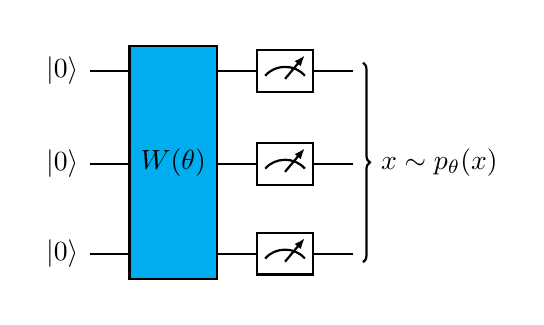
\begin{tikzpicture}
			\node{
				\begin{quantikz}
					\lstick{$\ket{0}$} & \gate[wires = 3, style={fill=cyan}]{W(\theta)} & \meter{} & \qw\rstick[wires=3]{$x \sim p_\theta (x)$} \\
					\lstick{$\ket{0}$} & & \meter{} & \qw \\
					\lstick{$\ket{0}$} & & \meter{} & \qw
				\end{quantikz}
			};
		\end{tikzpicture}
		\caption{Variational quantum algorithm for unsupervised approach}
		\label{vqa unsupervised}
	\end{figure}
\end{center}
So it is possible to notice that the only differences between the unsupervised and supervised model are two: the absence of embedding layer and data basis for measurement instead of the output basis.Probabilistic quantum model is strictly correlated to deteminsitc one due to the fact that $p_\theta(x) = |\braket{x|\psi(\theta)}|^2$ can be even seen as $\bra{x}(\ket{\psi(\theta)} \bra{\psi(\theta)}) \ket{x}$ with basis measurement of $\mathcal{M} = \ket{\psi(\theta)} \bra{\psi(\theta)}$. This is important because it define a clear connection betwenn the insights on designs applied. Futhermore it is possible to notice that \acrshort{vqa} are generative models, but it is difficult to extract this distribution due to the measurements requried. Lastly unsupervised quantum models are even known as \textit{Born machines} from the Born rule that links quantum states and probability.
\subsubsection{Quantum models as linear combinations of periodic functions}
For generality it is possible to express the quantum circuit using in the model as an alternation between encoding an parametrized gates repeated for multiple layers as:
\begin{equation}\label{udecomp}
	U(x,\theta) = W_{N+1}(\theta) = \prod_{i = 1}^{N} S_i(x_i)W_i(\theta)
\end{equation}
embedding gate can be defined as having the form $S_i(x_i) = e^{-i x_i G_i} $ where $G_i$ without losing genrality can be assumed a diagonal operator $diag(\lambda_{i}^{1}, \dots, \lambda_{i}^{1} )$ with d dimension of Hilbert space. Then a theorem proven by \cite{Schuld_theorem} demonstrate the linear combination of such models.
\begin{theorem}
	Let $X \in \mathbb{R}^n$, $Y = \mathbb{R}$ and $f_\theta:X \to Y$ be a deterministic quantum model with a circuit $U(x,\theta)$ as defined in \ref{udecomp}. Accordingly the i-th  feature is encoded by gate $ e^{-i x_i G_i}$: Then $f_\theta$ can be written as 
	\begin{equation*}
		f_\theta(x) = \sum_{w_1 \in \Gamma_1} \dots \sum_{w_N \in \Gamma_N} c_{w_1 \dots w_n}(\theta) e^{iw_1 x_1} \dots e^{iw_N x_N}
	\end{equation*}
	with the frequency spectrum of the i-th feature, $i=1,\dots,N$ is given by 
	\begin{equation*}
		\Gamma_i = \{\lambda_{s}^{i} - \lambda_{t}^{i} | s, t \in {1, \dots,d} \}
	\end{equation*}
	This frequency spectrum is the set of all values produced by differences between
	any two eigenvalues of $G_i$ . We are guaranteed that $0\in\Gamma$, and for each $w \in \Gamma$	there is $-w \in \Gamma$ too with $c_w(\theta) = c_{-w}^{*}(\theta)$. This symmetry guarantees that $f_\theta$ is real-valued, and that the sum can be rewritten with cosine and sine functions.
\end{theorem}
This theorem is important because it tells that there is no linearity if only the variational cirucit is applied, the frequencies are defined by the embedding layer and weights are dependent on parameters and frequencies. This means that for an expressive \acrlong{vqa} the embedding and parameters layer must be repeated multiple times to have enough expressitivity.
This means that unfortunately non-linearity is not present on these circuits, unless measurement or specific gate are introduced as it will be seen later.
\subsubsection{Variational algorithm training}
As previously stated this type of cicruit is parametrized and the parameters are optimized by calculating a cost function and the gradient. Due to the fact that cost fucntion is dependendant in first place from output function and afterward to parameters, the chain rule needs to be applied obtaining the following equation:
\begin{equation}
	\frac{\partial C(\theta)}{\partial \mu} = \frac{\partial C(\theta)}{\partial f(\theta)} \frac{\partial f(\theta)}{\partial \mu} 
\end{equation}
This form has two components $\frac{\partial C(\theta)}{\partial f(\theta)}$ and $\frac{\partial f(\theta)}{\partial \mu}$ required to exactly calculate the differentiation. First one can be obtained using classical computation, while the second one cannot be evaluated using classical quantities because it depend directly on the quantum circuit.
In fact using the parameter-shift rules it possible to calculate the gradient of a quantum circuit compared to the parameters $\frac{\partial f(\theta)}{\partial \mu}$ , while for the other quantity library such as \textit{Tensorflow} and \textit{Pytorch} can apply \textbf{automatic differentiation} to approxiamte the result.\\
\begin{mydef}[parameter-shift rules]
Let $f_\mu = \braket{\mathcal{M}}_\mu$ be a quantum expectation value that depends on a classical parameter $\mu$. A parameter-shift rule is an identity of the form:
\begin{equation}
	\partial_\mu f_\mu = \sum_{i} a_i f_{\mu + s_i}
\end{equation}
where ${a_i}$ and ${s_i}$ are real scalar value.
\end{mydef}
As it can be noticed this formula is similar to the finite difference method which is:
\begin{equation*}
	\frac{\partial f_\theta}{\partial \mu} \approx \frac{f_\theta - f_{\theta + \Delta \theta}}{||\Delta \theta||}
\end{equation*}
the main difference is that \textbf{the parameter-shift rule method is able to estimate the analytic gradient, while the finite difference method focus on approximating it}. Furthermore the parameter-shift rule is not dependant on how big or small must be the variation in order to correctly calculate the gradient and requires very few evaluations.
There is a problem with the gradients of variational circuits, that is a significant presence of \textbf{barren plateaus}. This term refers to the fact that sometimes the cost function can presents zone where the gradient is highly probable to be zero leading to small variantons on gradient. Mathematically speaking this means that:
\begin{equation}\label{barren plateau}
	Var[\partial_\mu f_\mu] = 0
\end{equation} 
This is a problem for the correct optimization of parameters due to the fact that gradient is particularly small leading to a non global minimal solution or requiring a great amount of training time before actually leaving this zone. The \textbf{barren plateaus} are present in \acrlong{nn} and is something studied and discussed, but no real solution has been actually found to deal with it.
Difference between classical and quantum model is the fact that these regions are \textbf{\textit{exponentially more large}} on the quantum case as demonstrated by \cite{McClean_2018}. The paper furthermore explains that increasing the number of gates, referred even as layers due to repetition of specific gates, and qubits leads to an exponential decay on the variance. This is an ulterior motive for which the variational circuit that is defined must be the most shallow in order to avoid problems on trainability. There has been some strategy addressed to partially solve this problem such as initialization using correlated parametrized circuit as suggested by \cite{Grant_2019}, but this represent one of the major challenge to solve in order to use deepest circuits. A deeper and more detailed explaination can be found in \cite{Schuld2021vqa}.
\subsubsection{Variational algorithm as neural networks}
Variational circuits are sometimes called "quantum neural networks". This name is partially reasonable due some resemblance to classical neural network such as the optimization of parameters and structure linearity for deep learning. Problem is that these circuits does not express non-linearity unless particularly encoding strategy or measurement is applied. 
In a interesting wa, non-linear activation function can be obtained by applying different types of encoding with slight modifications as suggested by \cite{Schuld2021vqa}, but the papers to create the ansatz for reinforcement learning does not apply them. It would be intersting to see if these encoding may result in a better performance on future tests.
A possible schematic on how \acrlong{vqa} can be interpreted as \acrlong{nn} is given by figure \ref{vqa nn}.From this schematic it can be observed an important fact the only non-linearity present is due to the measurement applied at the end. To introduce more non-linearity gates such as \textit{depolarizing gates} and even \textit{noise} can be added, but this is not a complete solution. Furthermore it can be noticed how every gate applied can be associated to a layer o f the neural network.
Possible representation that can be used is to define a formalism linked to connectivity by generalizing a single qubit gate as:
\begin{equation*}
	W = \begin{bmatrix}
		z & u \\
		-u* & z*
	\end{bmatrix}
\end{equation*}
\begin{center}
	\begin{figure}[!h]
		\centering
		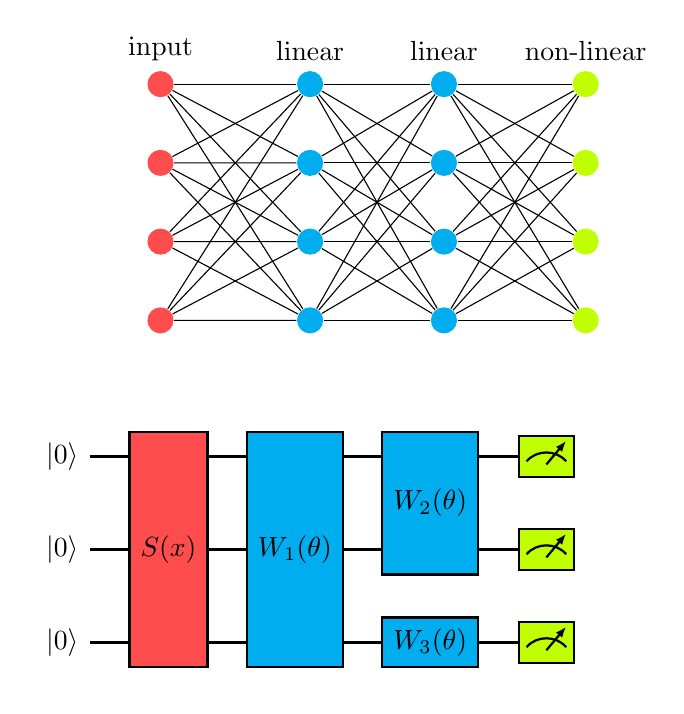
\begin{tikzpicture}
			\node[circle, fill=red!70, label={input}] (I-1) at (-0.2,-1) {};
			\node[circle, fill=cyan, label={linear}] (H-1) at (1.7cm,-1 cm) {};
			\node[circle, fill=cyan, label={linear}] (H_-1) at (3.4cm,-1 cm) {};
			\node[circle, fill=lime, label={non-linear}] (O-1) at (5.2cm,-1 cm) {};
			% Draw the input layer nodes
			\foreach \y in {2,...,4}{
				% This is the same as writing \foreach \name / \y in {1/1,2/2,3/3,4/4}
				\node[circle, fill=red!70] (I-\y) at (-0.2,-\y) {};
				\node[circle, fill=cyan] (H-\y) at (1.7cm,-\y cm) {};
				\node[circle, fill=cyan] (H_-\y) at (3.4cm,-\y cm) {};
				\node[circle, fill=lime] (O-\y) at (5.2cm,-\y cm) {};
			}
			\foreach \n in {1,..., 4}{
				\foreach \m in {1,..., 4}{
					\path (I-\n) edge (H-\m);
					\path (H-\n) edge (H_-\m);
					\path (H_-\n) edge (O-\m);
				}
			}
						
			\node[below = 10 mm of H-4](vc) {
				\begin{quantikz}
					\lstick{$\ket{0}$} & \gate[wires= 3, style={fill=red!70}]{S(x)} & \gate[wires = 3, style={fill=cyan}]{W_1(\theta)}& \gate[wires = 2, style={fill=cyan}]{W_2(\theta)} & \meter[style={fill=lime}]{}  \\
					\lstick{$\ket{0}$}& & & & \meter[style={fill=lime}]{} \\
					\lstick{$\ket{0}$}& & & \gate[style={fill=cyan}]{W_3(\theta)} & \meter[style={fill=lime}]{}
				\end{quantikz}
			};
		\end{tikzpicture}
		\caption{Variational quantum algorithm as a neural network}
		\label{vqa nn}
	\end{figure}
\end{center}
This matrix representation must respect the condition of normalization. In case the single qubit gate is applied on only one qubit, for example $i$, a multi-qubit representation can be defined by extending the previous definition:
\begin{equation*}
	W_i = \mathbbm{1} \otimes \dots \otimes \underbrace{W}_{i\;position} \otimes \dots \otimes \mathbbm{1}
\end{equation*}
The simbol $\mathbbm{1}$ refers to an identity matrix $2\times2$, this means that a single qubit gate applied leads to a sparse representation and the matrix able to represent any kind of operation applied on multiple qubits has shape $2^n \times 2^n$. This is interesting and gives a connection between layer of neural network with linear activation and vqa because both of them use matrix operations.
\subsubsection{Data reuploading}
As it was already explained before, the \acrlong{vqa} are linear except for the final points where measurement is applied. This can be problematic for the field of deep reinforcement due to significant presence of non-linear functions for the q-values and actor component. In order to introduce this non-linearity and deal with the \textbf{non-cloning} property of quantum computing a new type of ansatz has been defined: \textit{\textbf{data reuploading}}.
This concept has been introduced in the paper \cite{P_rez_Salinas_2020} and it wants to introduce non-linearity by reapplying the embedding layer multiple times in order to have a more composite function expressivity. So the strategy is to not use more qubits, but apply multiple layer increasing the depth of final circuit. This seems to work particularly well for reinforcement learning using simulators. Question is if this kind of depth would be able to run omn a quantum computer and will be a ble to achieve the same performance. This is something that may be required further work.
\subsection{Quantum Deep Q-learning applied to Cartpole} 
Now that \acrlong{vqa} has been explained it is now time to see the results obtained by applying qauntum models on the environment called Cartpole-v0. This is part of the library Open-AI gym (\cite{1606.01540}, \href{https://www.gymlibrary.ml/}{link}), which contains multiple environments used for benchmarking reinforcement learning algorithms.\\
The Cartpole environment is composed by a pole attached to a cart:
\begin{figure}[h]
	\centering
	\includegraphics[width=0.7\linewidth]{img/cartpole}
	\caption[Cartpole environment]{Cartpole environment of Open-AI gym}
	\label{fig:cartpole}
\end{figure}\\
The environment state is an array of 4 values representing: (position, velocity, pole angle, pole angular velocity). Position and angle are limited in value, while the others are not. The possible action that can be taken is a single value tha can be 0 or 1, which respectivelly means push left or right. The reward given by the environment is that for every step taken the total reward is increased by 1 even on termination. The conditions for which an episode is stopped are: the cartpole reaches extrems of the environment, angle pole is equal or greater than 12° or the number of steps taken is equal to 200.\\
The goal is to reach a reward greater or equal than 175 for 100 episodes. Technically when this condition is reached the training should be stopped, but it will be extended for 1000 episodes in order to check the stability and convergence of the algorithm. To confront the advantage between \acrlong{nn} and \acrlong{vqa} it will be counted the trend of reward, the number of episode taken to reach the goal, time taken and numbers of parameters.
This has been decided from reference of other papers that used this way to benchmark classical and quantum models.\\
\subsubsection{Ansatz for VQA}
Different ansatz have been used for this work, the starting point was form the paper \cite{Scholik_2022} which has a corresponfing github repository that can be used for the code.
Variational circuit proposed for the paper is based from the following layer:
\begin{figure}[!h]
	\centering
	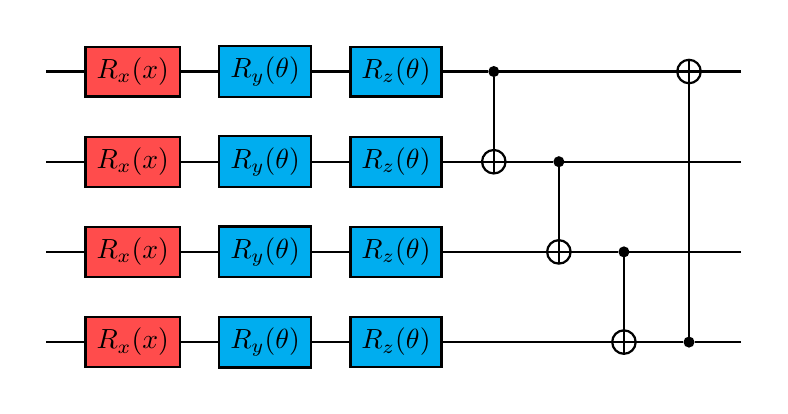
\begin{tikzpicture}
			\node(vq) {
				\begin{quantikz}
					\qw & \gate[style={fill=red!70}]{R_x(x)} & 	\gate[style={fill=cyan}]{R_y(\theta)}& \gate[style={fill=cyan}]{R_z(\theta)} & \ctrl{1} & \qw & \qw & \targ{} & \qw  \\
					\qw & \gate[style={fill=red!70}]{R_x(x)} & 	\gate[style={fill=cyan}]{R_y(\theta)}& \gate[style={fill=cyan}]{R_z(\theta)} & \targ{} & \ctrl{1} & \qw & \qw & \qw \\
					\qw & \gate[style={fill=red!70}]{R_x(x)} & 	\gate[style={fill=cyan}]{R_y(\theta)}& \gate[style={fill=cyan}]{R_z(\theta)} & \qw & \targ{} & \ctrl{1} & \qw & \qw \\
					\qw & \gate[style={fill=red!70}]{R_x(x)} & 	\gate[style={fill=cyan}]{R_y(\theta)}& \gate[style={fill=cyan}]{R_z(\theta)} & \qw & \qw & \targ{} & \ctrl{-3}  & \qw
				\end{quantikz}
			};
		\end{tikzpicture}
	\caption{Variational quantum algorithm for cartpole }
	\label{vqa dqn}
\end{figure}\\
As it can be seen, this kind of layer applies the data-reuploading approach already mentioned. This seems vital in order to achieve a good performance in respect to the classical one, for more detail please consult the paper. This kind of layer is repeated multiple times in order to achieve enough depth for the expresssivity required to approximate the best q-value function. The measurement applied at the end uses probabilistic approach, in fact due to the nature of cartpole a single action is required, go left or right, so in order to reduce the dimension output a measurement composed on two qubits corresponding to $Z \otimes Z$ is applied. After the measurement value with maximum probability is chosen and executed. In order to increase the performance a classical layer of weights on input and output is added, this leads to the folloring final structure.
\begin{figure}[!h]
	\centering
	\resizebox {1.1\linewidth} {!} {
	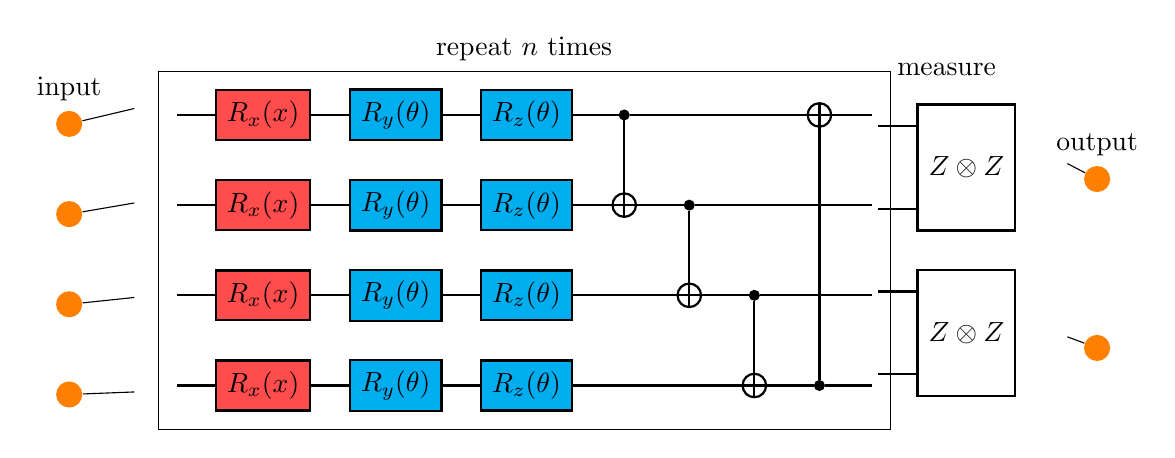
\begin{tikzpicture}
		\node[draw, label = {repeat $n$ times}](dqn) {
			\begin{quantikz}
				\qw & \gate[style={fill=red!70}]{R_x(x)} & 	\gate[style={fill=cyan}]{R_y(\theta)}& \gate[style={fill=cyan}]{R_z(\theta)} & \ctrl{1} & \qw & \qw & \targ{} & \qw   \\
				\qw & \gate[style={fill=red!70}]{R_x(x)} & 	\gate[style={fill=cyan}]{R_y(\theta)}& \gate[style={fill=cyan}]{R_z(\theta)} & \targ{} & \ctrl{1} & \qw & \qw & \qw \\
				\qw & \gate[style={fill=red!70}]{R_x(x)} & 	\gate[style={fill=cyan}]{R_y(\theta)}& \gate[style={fill=cyan}]{R_z(\theta)} & \qw & \targ{} & \ctrl{1} & \qw & \qw  \\
				\qw & \gate[style={fill=red!70}]{R_x(x)} & 	\gate[style={fill=cyan}]{R_y(\theta)}& \gate[style={fill=cyan}]{R_z(\theta)} & \qw & \qw & \targ{} & \ctrl{-3} & \qw
			\end{quantikz}
		};
		\node[right= -4mm of dqn, label = {measure}](measure) {
			\begin{quantikz}
				\qw & \gate[wires =2]{Z \otimes Z} \\
				\qw & \qw \\
				\qw & \gate[wires =2]{Z \otimes Z}\\
				\qw & \qw 
			\end{quantikz}
		};
		\node[circle, above left = -8mm and 10mm of dqn , fill=orange, label={input}] (I1) {};
		\node[circle, below = 8mm of I1 , fill=orange] (I2) {};
		\node[circle, below = 8mm of I2 , fill=orange] (I3) {};
		\node[circle, below = 8mm of I3 , fill=orange] (I4) {};
		\path (I1) edge (-4.95,1.8);
		\path (I2) edge (-4.95,0.6);
		\path (I3) edge (-4.95,-0.60);
		\path (I4) edge (-4.95,-1.8);
		\node[circle, above right = -15mm and 25mm of dqn , fill=orange, label={output}] (O1) {};
		\node[circle, below = 18mm of O1 , fill=orange] (O2) {};
		\path (6.9, 1.1) edge (O1);
		\path (6.9, -1.1) edge (O2);
	\end{tikzpicture}
}
	\caption{Final structure for cartpole}
	\label{dqn hybrid}
\end{figure}
The original implementation used as libraries pennylane and pytorch, this made the algorithm take around 11 hours for 5000 episodes. Due to the requirement of benchmarking the code has been rewritten using tensorflow quantum. This allowed a speedup by reducing the time required ...\\
By applying multiple runs and confronting the runs made by the quantum algorithm and different kind of neural network this result is obtained:
\begin{figure}[!h]
	\centering
	\includegraphics[width=\linewidth]{img/VQCNNcomparisonmedia}
	\caption[Benchmark of quantum and classical dqn]{In this image it has been used the mean and the variance of 10 runs of neural networks and vqa}
	\label{fig:vqcnncomparisonmedia}
\end{figure}\\
As it can be seen from the figure a neural network with the same number of vqa parameter is unable to reach the goal of cartpole and in order to have the same trend a neural network with 1256 parameters.\\
This means that a quantum advantage on the number of parameters and expressivity of the modes with few layers. The paper referenced is more expressive and even more detailed on all hyperparameters that has been tested, the configuration used for this benchmark is:
\begin{center}
	\begin{tabular}{|c|c|c|c|}
		\hline
		hyperparameter & NN(1256 params) & NN(48 params) & VQA \\
		\hline
		$\gamma$ & 0.99 & 0.99 & 0.99 \\
		\hline
		optimizer & Adam & Adam & Adam \\
		\hline
		batch size & 64 & 64  & 16 \\
		\hline
		learning rate & 0.001 & 0.001 & 0.01 \\
		\hline
		buffer memory & 100000 & 100000 & 10000 \\
		\hline
		$\epsilon$ start & 0.1 & 0.1 & 1 \\
		\hline
		$\epsilon$ decay & 0.99 & 0.99 & 0.99 \\
		\hline
		$\epsilon$ final & 0.001 & 0.001 & 0.01 \\
		\hline
		Loss & Smooth-L1 & Smooth-L1 & Smooth-L1 \\
		\hline
		neuron layers & (4,32)(32,32)(32,2) & (4,8)(8,2) & (4,)(2,)  \\
		\hline
		vqa layers & None & None & 5 \\
		\hline
	\end{tabular}
\end{center}
As it can be seen from the hyperpaprameters $\epsilon$ used for the $\epsilon$-greedy algorithm used is decreased from starting to ending value applying a formula called linear decay.\\
A better and more efficient ansatz was proposed by tensorflow quantum exactly for this kind of problem giving to the following structure of the \acrlong{vqa}:
\begin{figure}[h]
	\centering
	\includegraphics[width=0.8\linewidth]{img/tfq}
	\caption{Ansatz of variational circuit with data reuploading of the tensorflow quantum library}
	\label{fig:tfq}
\end{figure}\\
The differences between this kind of ansatz and \ref{dqn hybrid} are: the lack of classical weights input-output and most importantly the encoding layer is parametrized. This means that the expressivity of this model can be tuned by finding the parameters that are able to give the best encoding to find afterward best approximation.
%%%%%%%%%%%%%%%%%%%%%%%%%%%%%%%Important
%%from here i need my results
Now that the results of Cartpole has been showed proving that there can be a qantum advantage using less parameters, it is now change for another environment which is based on the robotic arm and can be a demonstration on the quantum capabilities applied on possible future industrial application.
\subsection{Variational quantum algorithm on robotic arm}
\subsubsection{Environment}
The previous environment is used for benchmarking and to have a partial view on the capability of this algorithm. It is now time to test it on something more difficult and with application on the industry: a robotic arm. This technology is applied in many field of industry such as: manufacturing, cars and many others.The environment that will be used to simulate a robotic arm has been created and offered from prof.Noah Klarmann from the university of Rosenheim who I would like to thank.This environment is formed of an arm composed of different links whose number can be defined, this influence both the space of state and action, with a randomic point which need to be reached by the arm using his extremis. The links are independent and can move on any direction with a fixed maximum velocity, this means that for every possible point that can be reached the number of steps required is not always the same.As it can be seen from this rendering:
\begin{figure}[h]
	\centering
	\includegraphics[width=0.45\linewidth]{img/quantum_robotic_arm_SAC_4182}
	\caption{Robotic arm with 2 links, the termination point of arm is green and the objective point is red}
	\label{fig:roboticarmsac}
\end{figure}\\
The total return is calculated every step taken, the value is negative for every step that the arm was unable to reach the determined point and is defined as the eukledian distance between arm termination and point. In case the arm is able to effectively reach the point a positive reward of +5 is given and the episode is considered ended. The termination conditions are two: the steps taken is equal to 250 or the point is reached. The state tuple is composed in case of 2 links: (target x, targe y, end effector x, end effector y, link angle 1, link angle 2) in case of more link the tuple increase considerinfg more angles. The action tuple has length equal to links and for the case of 2, it is : (link 1 velocity, link 2 velocity).There isn't an exact condition for which the environment is considered solved, but from multiple runs and afterward rendering the environment was decided to be considered solved when the mean reward was above 40 for the case of 2 links.
Differerently from the cartpole enviornment, robotic arm can be multidiscrete or continous and for application it was decided to use the continuos one and use the \acrfull{sac} by substituting a complete neural network approach with an hybrid which uses the \acrshort{vqa}.
\subsubsection{Quantum SAC}
A paper has been already published which uses a quantum \acrshort{sac} approach to solve the pendulum-v0 environment, the details can be found in \cite{https://doi.org/10.48550/arxiv.2112.11921}.
\begin{algorithm} \label{qsac}
	\caption{Variational Quantum Sac}
	\begin{algorithmic}
		\REQUIRE initial policy parameters $\theta$, initial action-value estimate parameters $\phi_1$ and $phi_2$, $\gamma$, $\alpha$, $\rho$, empty experience replay $D$.
		\STATE Initialize the hybrid quantum-classical policy network with $\theta$.
		\STATE Initialzie two action value networks with $\phi_1$ and $phi_2$ respectively.
		\STATE Set target-action value networks parameters: $\phi_{targ, 1} \leftarrow \phi_1$ and $\phi_{targ, 2} \leftarrow \phi_1$.
		\FOR{each time-step}
			\STATE Observe state $S$, select action $A \sim \pi_{\theta}(\cdot |S)$ and execute $A$ in the environment.
			\STATE Observe next state $S'$, reward $R$, and binary done signal $d$ to indicate whether $S'$ is terminal state or not.
			\STATE Store $(S,A,R,S',d)$ in $D$.
			\STATE Reset the environment if $d=1$.
			\STATE Sample a batch of transitions $B = {(S,A,R,S',d)}$ from $D$ randomly.
			\STATE Compute target values $y(R,S',d) = R + \gamma (1-d) (min_{i=1,2}Q_{\phi_{targ,i}} (S',A') - \alpha \log \pi_{\theta}(A',S'))$ where $A' \sim \pi(\cdot,S')$.
			\STATE Update $\phi_i$ by minimizing: $\mathbb{E}_B [(Q_{\phi_i}(S,A) - y(R,S',d))^2]$ for $i = 1,2$.
			\STATE Update $\theta$ by maximizing: $\mathbb{E}_B [min_{i=1,2} Q_{\phi_i}(S,\tilde{A}_\theta) - \alpha \log \pi_{\theta}(\tilde{A}_\theta|S)]$.
			\STATE Do a soft update for target action-value networks: $\phi_{targ,i} \leftarrow \rho \phi_{targ,i} + (1-\rho)\phi_i$ for $i=1,2$.
		\ENDFOR
	\end{algorithmic}
\end{algorithm}\\
So from this algorithm it is possible to understand that there 5 components necessary: an actor policy, two action-value approximator and others two called target action-value approximator.
The reason for which it is necessary the target components is similar to the \acrshort{dqn} case, due to the fact that usually two consecutive states are not independent and requiring action-values to be it in order to correctly update the weights an independent copy is required.
The reason for which both of action and target components is double can be explained from other advances of \acrshort{dqn} which showed that using two components and taking minimum of the two improves performance and stability.
The final component which is an actor policy, for the case of \acrshort{sac} this component will output two values: mean and variance of a gaussian distribution. From this the action will be sampled randomically meaning that this approach is statistical, it can be converted to deterministic by using the mean extracted from the component.\\
This policy actor in the paper is defined as a quantum-classic hybrid approach that differently form \acrshort{dqn} tries to incorporate \acrlong{nn} layers and \acrlong{vqa}. An image showing the actual structure is present on the paper:
\begin{figure}[h]
	\centering
	\includegraphics[width=0.6\linewidth]{img/qsac}
	\caption{Hybirid actor policy architecture, image taken from \cite{https://doi.org/10.48550/arxiv.2112.11921}}
	\label{fig:qsac}
\end{figure}\\
So of the 5 component present on this algorithm only one uses the \acrshort{vqa} with \acrshort{nn}, this can be a limitation and afterword the results using an algorithm for which every component applies it. All the test showed, are the ones with an environment that uses 2 links, this is due to a lack of time and resources. 
\subsubsection{Results with hybrid actor}
Using the previous ansatz and algorithm it was decide to apply the hybrid architecture only on the actor component applying 4 and 5 layers giving a total of respectively 100 and 112 parameters.
To confront it with a \acrshort{nn} two test were carried out using 149 and 164 parameters leading to this interesting plot. The runs could not be repeated for the lack of time and resources required, in fact the hybrid architecture took almost 19 hours to reach this point. Even if the classical one took only 4, in order to benchmark them it would require at least 1 week and as it will be noticed this kind of solution is not optimal as it will be later noticed.
One of the reasons for which this runs weren't repeated multiple times is the time and resources required, in  fact using multiple cpu or applying in the future on a gpu may reduce significantly this time. Unfortunately on the time of writing this is not possible, but it may be applied in the future.\\
Confronting result obtained using hybrid and classical components gives:  
\begin{figure}[H]
	\centering
	\includegraphics[width=0.8\linewidth]{"img/VQA and classic actor"}
	\caption{Moving average with time window of 30 with mean and standard deviation of the trend.}
	\label{fig:vqa-and-classic-actor}
\end{figure}
From this an interesting fact can be noticed: all of the test have more or less the same trend and reach the same return at around 150000 steps. As can be seen the hybrid algorithm present an higher steep curve confronting to the classical ones and is able to reach the plateau slightly faster, but there isn't a clear qurnum advantage due to the similar number of parameters and time step taken.
This is quite suspicious and could mean that the critical component may nit be the acto, but the critic. To confirm this suspect notice the plot of only the actor component that use \acrlong{nn}:
\begin{figure}[H]
	\centering
	\includegraphics[width=0.8\linewidth]{"img/classics actor"}
	\caption{Plot of the runs that uses neural netowrks for all the components.}
	\label{fig:classics-actor}
\end{figure}
As it can be noticed an increase on the number of parameters doesn't determine a great variation, instead if a plot using the hybrid algorithm and confronting them by resusing the same architecture a plot is obtained:
\begin{figure}[H]
	\centering
	\includegraphics[width=0.8\linewidth]{"img/VQA critic reduced"}
	\caption{Plot confronting vqa with reduced parameters of critic and previous ones.}
	\label{fig:vqa-critic-reduced}
\end{figure}
\vspace{0.5cm}
So effectively the most impacting component on the ability of reaching the goal of this algorithm is not the actor, but are the critic ones! Here can be found the table containing information on the structure of components where it can be noticed that except the number of params the test runs uses almost everywhere the same exact hyperparmeters:
\newline
\vspace{0.2cm}
\newline
\begin{tabular}{|c|c|c|}
	\hline
	Hyperparameters & VQA 4 layers & VQA 5 layers  \\
	\hline
	$\gamma$ & 0.99 & 0.99  \\
	\hline
	$\alpha$ & 0.2 & 0.2  \\
	\hline
	learning rate & 0.0003 & 0.0003  \\
	\hline
	memory size & 1000000 & 1000000   \\
	\hline
	optimizer & Adam & Adam  \\
	\hline
	actor neurons  & (6, VQA, (1,1)) & (6, VQA, (1,1))  \\
	\hline
	actor act. func. & (linear,relu,linear) & (linear,relu,linear) \\
	\hline
	actor params & 100 & 112 \\
	\hline
	critic neurons & (8,64,64,1) & (8,64,64,1)  \\
	\hline
	critic act. func. & (linear,relu,relu,linear) & (linear,relu,relu,linear) \\
	\hline
	critic params & 4608 & 4608 \\
	\hline
	total params & 18532 & 18544 \\
	\hline
\end{tabular}
\newline
\vspace{0.5 cm}
\newline\begin{tabular}{|c|c|c|}
	\hline
	Hyperparameters & VQA 4 layers reduced & VQA 5 layers reduced  \\
	\hline
	$\gamma$ & 0.99 & 0.99   \\
	\hline
	$\alpha$ & 0.2 & 0.2   \\
	\hline
	learning rate & 0.0003 & 0.0003   \\
	\hline
	memory size & 1000000 & 1000000   \\
	\hline
	optimizer & Adam & Adam  \\
	\hline
	actor neurons  & (6, VQA, (1,1)) & (6, VQA, (1,1))  \\
	\hline
	actor act. func. & (linear,relu,linear) & (linear,relu,linear) \\
	\hline
	actor params & 100 & 112  \\
	\hline
	critic neurons & (8,16,16,1) & (8,16,16,1)  \\
	\hline
	critic act. func. & (linear,relu,relu,linear) & (linear,relu,relu,linear) \\
	\hline
	critic params & 384 & 384\\
	\hline
	total params & 1636 & 1648\\
	\hline
\end{tabular}
\newline
\vspace{0.5 cm}
\newline
\begin{tabular}{|c|c|c|}
\hline
Hyperparameters & Actor NN 149 & Actor NN 164 \\
\hline
$\gamma$  & 0.99 & 0.99 \\
\hline
$\alpha$ & 0.2 & 0.2 \\
\hline
learning rate  & 0.0003 & 0.0003 \\
\hline
memory size  & 1000000 & 1000000 \\
\hline
optimizer  & Adam & Adam \\
\hline
actor neurons & (6,24,(1,1)) & (6,26,(1,1)) \\
\hline
actor act. func. & (linear,relu,linear) & (linear,relu,linear) \\
\hline
actor params & 149 & 164 \\
\hline
critic neurons & (8,64,64,1) & (8,64,64,1) \\
\hline
critic act. func. & (linear,relu,relu,linear) & (linear,relu,relu,linear) \\
\hline
critic params & 4608 & 4608 \\
\hline
total params  & 18581 & 18596 \\
\hline
\end{tabular}\\
\\
The reason for which the toal parameters is so high links to the fact that there are 4 critic components that are required in order for the algorithm to work and learn.
\subsubsection{Results with hybrid actor and critic}
Now that the previous test have demonstrated that critic is the component that determines the most on performace the following test will use the hybrid algorithm used for the actor and apply it on critic. During the first tests we noticed that the previous structure used for actor, isn't good for the critic due to maybe a high non-linearity of the map required. For this reason the previous structure was modifided by adding a hidden layer before the output to increase the expressivity of non-linearity. This is the schematic:
\begin{figure}[!h]
	\centering
	\resizebox {1.0\linewidth} {!} {
	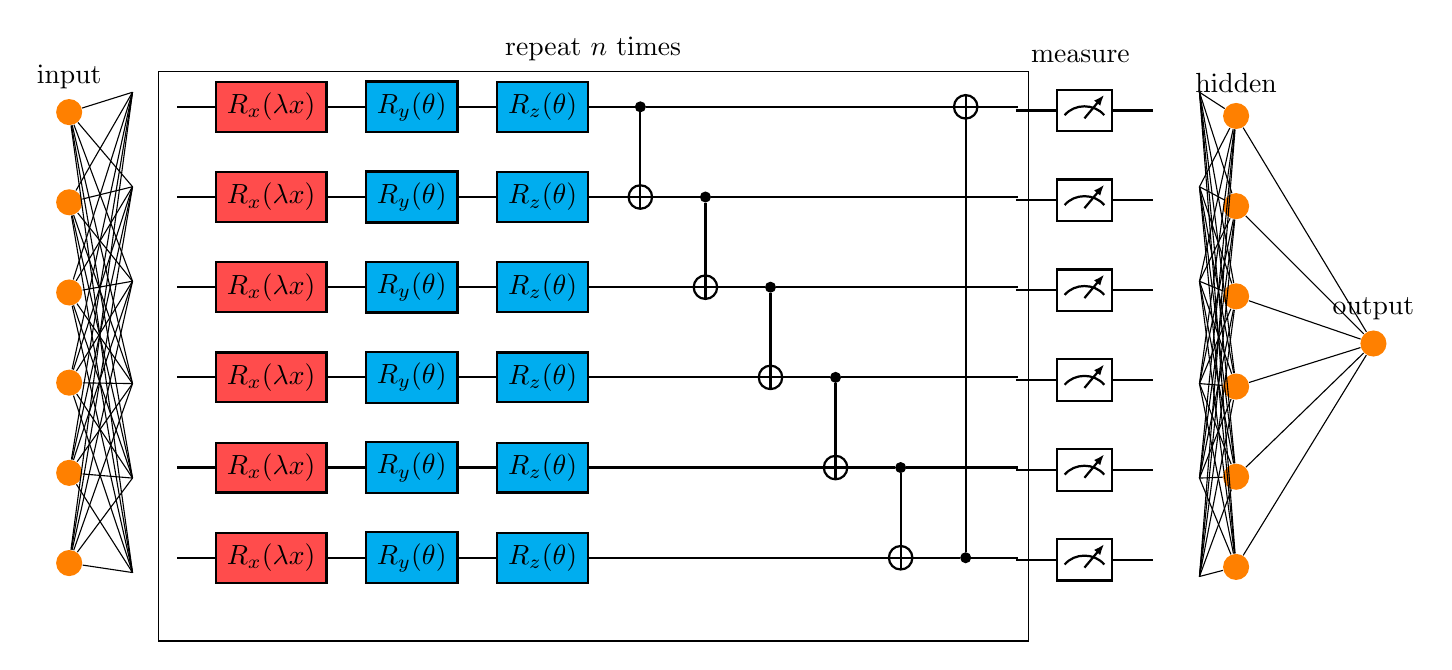
\begin{tikzpicture}
		\node[draw, label = {repeat $n$ times}](vqc) {
			\begin{quantikz}
				\qw & \gate[style={fill=red!70}]{R_x(\lambda x)} & 	\gate[style={fill=cyan}]{R_y(\theta)}& \gate[style={fill=cyan}]{R_z(\theta)} & \ctrl{1} & \qw & \qw & \qw & \qw & \targ{} & \qw \\
				\qw & \gate[style={fill=red!70}]{R_x(\lambda x)} & 	\gate[style={fill=cyan}]{R_y(\theta)}& \gate[style={fill=cyan}]{R_z(\theta)} & \targ{} & \ctrl{1} & \qw & \qw & \qw & \qw & \qw \\
				\qw & \gate[style={fill=red!70}]{R_x(\lambda x)} & 	\gate[style={fill=cyan}]{R_y(\theta)}& \gate[style={fill=cyan}]{R_z(\theta)} & \qw & \targ{} & \ctrl{1} & \qw & \qw & \qw & \qw \\
				\qw & \gate[style={fill=red!70}]{R_x(\lambda x)} & 	\gate[style={fill=cyan}]{R_y(\theta)}& \gate[style={fill=cyan}]{R_z(\theta)} & \qw & \qw & \targ{} & \ctrl{1} & \qw & \qw & \qw \\
				\qw & \gate[style={fill=red!70}]{R_x(\lambda x)} & 	\gate[style={fill=cyan}]{R_y(\theta)}& \gate[style={fill=cyan}]{R_z(\theta)} & \qw & \qw & \qw & \targ{} & \ctrl{1} & \qw & \qw \\
				\qw & \gate[style={fill=red!70}]{R_x(\lambda x)} & 	\gate[style={fill=cyan}]{R_y(\theta)}& \gate[style={fill=cyan}]{R_z(\theta)} & \qw & \qw & \qw & \qw & \targ{} & \ctrl{-5} & \qw \\
			\end{quantikz}
		};
		\node[right = -4mm of vqc, label = {measure}](measure) {
			\begin{quantikz}
				\qw & \meter{} & \qw \\
				\qw & \meter{} & \qw \\
				\qw & \meter{} & \qw \\
				\qw & \meter{} & \qw \\
				\qw & \meter{} & \qw \\
				\qw & \meter{} & \qw \\
			\end{quantikz}
		};
		\node[circle, above left = -6.5mm and 10mm of vqc , fill=orange, label={input}] (I1) {};
		\node[circle, below = 8mm of I1 , fill=orange] (I2) {};
		\node[circle, below = 8mm of I2 , fill=orange] (I3) {};
		\node[circle, below = 8mm of I3 , fill=orange] (I4) {};
		\node[circle, below = 8mm of I4 , fill=orange] (I5) {};
		\node[circle, below = 8mm of I5 , fill=orange] (I6) {};
		\foreach \i in {1,2,3,4,5,6}{
			\path (I\i) edge (-5.85,3.35);
			\path (I\i) edge (-5.85,2.15);
			\path (I\i) edge (-5.85,0.95);
			\path (I\i) edge (-5.85,-0.35);
			\path (I\i) edge (-5.85,-1.55);
			\path (I\i) edge (-5.85,-2.75);
		}
		\node[circle, above right = -6.8mm and 8mm of measure , fill=orange, label={hidden}] (H1) {};
		\node[circle, below = 8mm of H1 , fill=orange] (H2) {};
		\node[circle, below = 8mm of H2 , fill=orange] (H3) {};
		\node[circle, below = 8mm of H3 , fill=orange] (H4) {};
		\node[circle, below = 8mm of H4 , fill=orange] (H5) {};
		\node[circle, below = 8mm of H5 , fill=orange] (H6) {};
		\foreach \i in {1,...,6}{
			\path (H\i) edge (7.7,3.35);
			\path (H\i) edge (7.7,2.15);
			\path (H\i) edge (7.7,0.95);
			\path (H\i) edge (7.7,-0.35);
			\path (H\i) edge (7.7,-1.55);
			\path (H\i) edge (7.7,-2.8);
		}
		\node[circle, below right = 15mm and 15mm of H2, fill=orange, label={output}] (O1) {};
		\foreach \i in {1,...,6}{
			\path (H\i) edge (O1);
		}
	\end{tikzpicture}	
	}
	\caption{Structure for critic hybrid}
	\label{critic hybrid}
\end{figure}\\
As it can be seen from the plot \ref{fig:fully_vs_partial_quantum} by converting all components to hybrid architecture it was able to have a performance veery similar to the ones with only hybrid actor. As it will be seen later this means that a smaller component that uses few parameters is able to reach the same performance of one with more on the Neural network. Reason for which this line is interrupted after only 250000 steps is maily due to the high time required, in fact to reach that step the fully hybrid algorithm took more than a week and after concluding that the algorithm was performing very similarly to the actor hybrid it was stopped.\\
\begin{figure}[H]
	\centering
	\includegraphics[width=1.0\linewidth]{"img/fully_vs_partial_quantum"}
	\caption{Comparision between only actor hybrid and all components hybrid.}
	\label{fig:fully_vs_partial_quantum}
\end{figure}
Afterward to have a detailed cased for which multiple configuration with different size of the neural network were conducted in order to understand what kind of advantage was expected to confront the run of all-hybrid components and all neural networks. As it can be noticed from \ref{fig:all-classical-results} increasing the size of \acrlong{nn} and keeping the actor equal for all runs doesn't mean that there is an increase on performance and unfortunately the run that uses the least number of neurons is not able to reach the objective to have a score at least -40 as average. The choice on using 21 neurons is not casual, but it has been decided in order to have a similar number of parameters equal to the run that uses all hybrid components.
\begin{figure}[H]
	\centering
	\includegraphics[width=0.9\linewidth]{"img/All classical results"}
	\caption{All classical runs with an actor component of 149 parameters}
	\label{fig:all-classical-results}
\end{figure}
\begin{figure}[H]
	\centering
	\includegraphics[width=0.9\linewidth]{"img/Best classical vs all hybrid results"}
	\caption{Plot of best classical runs and all-hybrid}
	\label{fig:best-classical-vs-all-hybrid-results}
\end{figure}
\newpage

So by looking at \ref{fig:best-classical-vs-all-hybrid-results} an important result can be obtained, the all-hybrid run is able to reach a similar performance of all neural networks components that use an higher number of neurons to reach the objective with a similar trend and time steps required. \textbf{But if the neural network model uses a similar parameter number of all-hybrid model then it will not be able to reach the objective}.


	\section{Conclusion}
\subsection{Results obtained}
So in this thesis after a first dedicated to introduce the basis of \acrlong{drl} and quantum mechanics it was later presented the \acrlong{vqa} to simulate and replace \acrlong{nn}, observing what kind of advantage was possible to obtain in the context of reinforcement learning.
In order to understand if there was a quantistic advantage and on which aspect was present the ansatz proposed in the paper \cite{Scholik_2022} was tested as a quantum variation of the \acrlong{dqn} on Cartpole environment.\\
In order to compare it, a model with neural networks was runned with the most number of hyperparameters equal between the two. From results obtained and plot \ref{fig:vqcnncomparisonmedia} it was demonstrated that an effective advantage was obtained: an impressive smaller number of parameters was required to reach the objective and a neural network with the same number of weights was unable to do it.\\
This suggested that there is a more powerful expressivity and approximation capability compared to the neural network in this case. Unfortunately such kind of environment is extremely simple to solve and doesn't completely demonstrate this kind of ability and extension to more complex cases.\\
For this reason and to use the possible advantages and application on the industry a different  environment was tested: the robotic arm. This required to change the algorithm used previously due to continous state and actions which the \acrshort{dqn} is unable to deal for its discrete nature.\\
The new algorithm that was used is called \acrfull{sac}, differently from the \acrshort{dqn} it is policy gradient based and uses 5 components to learn. These are: actor policy which must calculate the mean and standard deviation, 2 action-values and 2 target action values that must update policy and approximate the correct functions in order to learn and work.
From a previous paper \cite{https://doi.org/10.48550/arxiv.2112.11921} it was defined a partial quantum \acrshort{sac} which demonstrated an advantage on the number of parameters by using an hybrid actor component. From the test conducted later on and in particular from plot \ref{fig:vqa-critic-reduced} an important conclusion was extrapolated: the critical component  that determines the performance of algorithm are action-values components.
So for this conclusion another run using all component as hybrid was conducted with an additional classical layer for the critical components in order to introduce enough non-linearity. Furthermore more test using all components leveraging neural networks were runned increasing every time the dimension of neurons on hidden layers.
Confronting the trend on plott \ref{fig:best-classical-vs-all-hybrid-results} it was noticed that in order to have a similar trend for the classical and hybrid run, it was necessary a number of parameters between 7 to 100 times and not always the steps required was similar. 
Furthermore running an example were all components using neural network has the same parameters number of hybrid, this model was unable to reach the goal of environment suggesting a quantum advantage on the number of parameters required and ability of expressivity useful for industrial applications.
\subsection{Future directions}
Possible future directions that should be interesting to take are:
 \begin{itemize}
	\item applies multiple runs on the hybrid algorithm possibly reducing the time required to run.
	\item introduce the noise on algorithms execution to understand the possible non-linearity and performance impacts on the ability to learn and difference on weights.
	\item develop better ansatz for the \acrshort{vqa} in order to reduce the dependence of non-linearity by neural networks layers and minimize the depth of circuit.
	\item test this \acrshort{vqa} on a real quantum computing using the parameter-shift method to calculate the gradients and use it later on a CPU to optimize the parameters showing performance and time reduction compared to this run on a simulators.
	\item test this algorithms on multiple environments to see if are better or worse compared to "classical" ones.
	\item extending the introduction of \acrshort{vqa} on other algorithms of \acrshort{drl} such as PPO, DDPG to confirm quantum advantage.
\end{itemize}
	\printbibliography[
	heading=bibintoc,
	title={Bibliography}
	]
\end{document}